\newpage
\clearpage

\section{Resultados e Discussões}
\label{results}
Neste capítulo, dedicado a Resultados e Discussões, serão apresentados e analisados os resultados dos experimentos realizados no transcurso deste estudo, acompanhados de uma reflexão criteriosa sobre os dados obtidos. Nesta etapa, será possível, portanto, avaliar a eficácia dos métodos que foram propostos e implementados, além de discutir as ideias futuras de implementação e as perspectivas coletadas para a evolução do tema em questão.

A estrutura do capítulo é delineada em seções que facilitam a compreensão dos resultados de acordo com o contexto do experimento aplicado. Na Seção \ref{results:class}, será discutido sobre os experimentos realizados prioritariamente para a tarefa de classificação. Esses experimentos iniciais foram fundamentais para balizar as análises e refinamentos subsequentes da técnica proposta.

Na sequência, a Seção \ref{results:semantic} irá abordar os resultados obtidos nos experimentos que se destinam diretamente à área de segmentação, que constitui o núcleo da aplicação da técnica proposta. Aqui, expandiremos o foco para a parcela mais crítica de nossa pesquisa, apresentando a eficácia de nosso método na tarefa de segmentação semântica de imagens.

Por fim, na Seção \ref{result:final} proporcionaremos as considerações finais em relação as seções anteriores, salientando as implicações dos resultados no campo de estudo do trabalho.

\subsection{Resultados da Classificação de Imagens}
\label{results:class}
Os experimentos e resultados desta seção fornecem valiosas percepções sobre o desempenho do método BPCAPooling em comparação com as estratégias de \textit{pooling} convencionais (\textit{Avg Pooling} e \textit{Max Pooling}) \citep{Ozdemir2023Avg-topk:Networks} quando aplicados na arquitetura VGG-16 para a tarefa de classificação.

Ao analisar o desempenho do modelo treinado no conjunto de dados CIFAR 100 utilizando o método proposto, observamos uma tendência indesejada. Este modelo apresentou a maior perda e a menor precisão quando comparado aos modelos utilizando os métodos \textit{Avg Pooling} e \textit{Max Pooling} no processo de descongelamento do terceiro bloco convolucional. Os resultados são evidenciados na Tabela \ref{results:class:tab:1}, que ilustra os desempenhos durante a fase de aquecimento do processo de \textit{fine-tuning}.

\begin{table}[H]
    \centering
    \caption{Resultados da fase de aquecimento de VGG-16 aplicada no conjunto de dados CIFAR 100.}
    \label{results:class:tab:1}
    \resizebox{0.6\textwidth}{!}{
    \begin{tabular}{l|c|c}
        \textbf{Método de \textit{Pooling}} & \textbf{Acurácia (\%)} & \textbf{\textit{Loss}}   \\
        \hline
        \textit{Avg Pooling}               & 36.300                 & 2.7309          \\
        BPCAPooling                        & 14.471                 & 3.7645          \\
        \textit{Max Pooling}               & \textbf{39.857}        & \textbf{2.0481}
    \end{tabular}}

    \vspace*{1 cm}
    Fonte: do próprio autor.
\end{table}

Mesmo após a conclusão do processo de \textit{fine-tuning} completo, o modelo treinado com a técnica BPCAPooling apresenta resultados inferiores, conforme evidenciado na Tabela \ref{results:class:tab:2}. Os métodos Max Pooling e Avg Pooling continuam a demonstrar uma superioridade significativa em relação ao método BPCAPooling. Os resultados mais promissores foram obtidos pela arquitetura VGG-16 com o método Max Pooling. A análise detalhada dos motivos subjacentes a essa discrepância será discutida na Seção \ref{results:class:datasets}.

\begin{table}[H]
    \centering
    \caption{Resultados por fase de \textit{fine-tuning} de VGG-16 aplicada no conjunto de dados CIFAR 100.}
    \label{results:class:tab:2}
    \resizebox{1\textwidth}{!}{
    \begin{tabular}{l|l|l|l|l|l|l|l|l}
    \multicolumn{1}{c|}{\textbf{Método de \textit{Pooling}}} & \multicolumn{2}{c|}{\textbf{Aquecimento}}                                          & \multicolumn{2}{c|}{\textbf{Bloco 5}}                                          & \multicolumn{2}{c|}{\textbf{Bloco 4}}                                          & \multicolumn{2}{c}{\textbf{Bloco 3}}                                          \\
    \cline{2-9}
    \multicolumn{1}{c|}{\textbf{}}                & \multicolumn{1}{c|}{\textbf{Acurácia(\%)}} & \multicolumn{1}{c|}{\textbf{\textit{Loss}}} & \multicolumn{1}{c|}{\textbf{Acurácia(\%)}} & \multicolumn{1}{c|}{\textbf{\textit{Loss}}} & \multicolumn{1}{c|}{\textbf{Acurácia(\%)}} & \multicolumn{1}{c|}{\textbf{\textit{Loss}}} & \multicolumn{1}{c|}{\textbf{Acurácia(\%)}} & \multicolumn{1}{c}{\textbf{\textit{Loss}}} \\
    \hline
    \textit{Avg Pooling}                                   &                                    36.300 &                            2.7309 &                                    39.340 &                            2.4971 &                                    41.371 &                            2.2958 &                                    42.371 &                            2.2364 \\
    BPCAPooling                                            &                                    14.471 &                            3.7645 &                                    15.185 &                            3.6677 &                                    16.229 &                            3.6020 &                                    17.543 &                            3.5121 \\
    \textit{Max Pooling}                                   &                                    39.857 &                            2.0481 &                                    43.671 &                            1.7166 &                                    45.100 &                            1.5448 &                                    \textbf{46.071} &                            \textbf{1.4862} 
    \end{tabular}}

    \vspace*{1 cm}
    Fonte: do próprio autor.
\end{table}

Para o conjunto de dados \textit{Food}-101, os resultados não divergiram muito dos obtidos no primeiro conjunto de dados. Durante a fase inicial do treinamento, os resultados do método proposto já se mostraram desafiadores em comparação aos outros métodos, como pode ser observado na Tabela \ref{results:class:tab:3}.

\begin{table}[H]
    \centering
    \caption{Resultados da fase de aquecimento de VGG-16 aplicada no conjunto de dados \textit{Food}-101.}
    \label{results:class:tab:3}
    \resizebox{0.6\textwidth}{!}{
    \begin{tabular}{l|c|c}
        \textbf{Método de \textit{Pooling}} & \textbf{Acurácia (\%)} & \textbf{\textit{Loss}}   \\
        \hline
        \textit{Avg Pooling}               & 41.290                 & 2.4042          \\
        BPCAPooling                        & 3.858                  & 4.7057          \\
        \textit{Max Pooling}               & \textbf{41.623}        & \textbf{2.3718}
    \end{tabular}}

    \vspace*{1 cm}
    Fonte: do próprio autor.
\end{table}

No contexto da aplicação do processo de \textit{fine-tuning}, observa-se consistentemente que o modelo de \textit{pooling} proposto demonstrou desempenho inferior em todas as fases quando comparado ao melhor método, que continuou sendo a junção de VGG-16 com \textit{Max Pooling}, conforme ilustrado na Tabela \ref{results:class:tab:4}.

\begin{table}[H]
    \centering
    \caption{Resultados por fase de \textit{fine-tuning} de VGG-16 aplicada no conjunto de dados \textit{Food}-101.}
    \label{results:class:tab:4}
    \resizebox{1\textwidth}{!}{
    \begin{tabular}{l|l|l|l|l|l|l|l|l}
    \multicolumn{1}{c|}{\textbf{Método de \textit{Pooling}}} & \multicolumn{2}{c|}{\textbf{Aquecimento}}                                          & \multicolumn{2}{c|}{\textbf{Bloco 5}}                                          & \multicolumn{2}{c|}{\textbf{Bloco 4}}                                          & \multicolumn{2}{c}{\textbf{Bloco 3}}                                          \\
    \cline{2-9}
    \multicolumn{1}{c|}{\textbf{}}                & \multicolumn{1}{c|}{\textbf{Acurácia(\%)}} & \multicolumn{1}{c|}{\textbf{\textit{Loss}}} & \multicolumn{1}{c|}{\textbf{Acurácia(\%)}} & \multicolumn{1}{c|}{\textbf{\textit{Loss}}} & \multicolumn{1}{c|}{\textbf{Acurácia(\%)}} & \multicolumn{1}{c|}{\textbf{\textit{Loss}}} & \multicolumn{1}{c|}{\textbf{Acurácia(\%)}} & \multicolumn{1}{c}{\textbf{\textit{Loss}}} \\
    \hline
    BPCAPooling                                   &                                    3.8586 &                            4.7057 &                                    4.3395 &                            4.6632 &                                    4.4130 &	                           4.4404 &                                    3.423  &	                           4.5187 \\
    Max Pooling                                   &                                    41.623 &                            2.3718 &                                    49.471 &                            \textbf{2.2033} &                                    \textbf{50.080} &                            2.3745 &                                    50.031 &                            2.4335 
    \end{tabular}}

    \vspace*{1 cm}
    Fonte: do próprio autor.
\end{table}

Na Tabela \ref{results:class:tab:4}, observa-se um comportamento distinto em comparação ao primeiro conjunto de dados. Os resultados de maior acurácia estão representados no quarto bloco, não no último bloco adicionado, o que levanta questionamentos sobre a influência desse bloco, assunto que será discutido na Seção \ref{results:class:datasets}.

Em relação ao custo computacional, observou-se que o método proposto, desenvolvido utilizando o \textit{framework} Tensorflow, exigiu um processamento considerável, resultando em desempenho mais lento durante os testes devido ao aumento da complexidade. Por exemplo, no caso do conjunto de dados CIFAR 100, com o descongelamento de blocos e $700$ épocas utilizando a configuração de \textit{hardware} de referência, os métodos \textit{Max Pooling} e \textit{Avg Pooling} levaram cerca de $7$ horas para serem executados. Em contrapartida, o BPCAPooling exigiu aproximadamente $19$ horas, cerca de $2,71$ vezes mais tempo, ressaltando que o conjunto de dados CIFAR 100 é otimizado para processamento em GPU.

Resultados semelhantes foram observados no conjunto de dados \textit{Food}-101, onde \textit{Max Pooling} e \textit{Avg Pooling} levaram cerca de $33$ horas para o processo de treinamento e validação, enquanto o BPCAPooling demandou aproximadamente \textit{38} horas. O aumento no tempo de processamento se deve principalmente ao tamanho maior das imagens. É importante mencionar que este conjunto de dados não está otimizado para processamento em GPU, o que resulta em um desempenho do \textit{hardware} abaixo do ideal.

Apesar dos resultados inesperados em relação ao método BPCAPooling, alguns \textit{insights} puderam ser extraídos das fases de treinamento e validação. Esses pontos de introspecção serão abordados a seguir nesta seção, juntamente com informações sobre a influência da aplicação desse método nas características específicas dos diferentes conjuntos de dados (Seção \ref{results:class:datasets}), a exploração da interpretabilidade das classificações utilizando a abordagem LIME e conceitos de preservação de espacialidade (Seção \ref{results:class:lime}), e sugestões para possíveis melhorias no desempenho do modelo atual (Seção \ref{results:class:future}).


\subsubsection{Diferença de conjuntos de dados}
\label{results:class:datasets}
A utilização de múltiplos conjuntos de dados foi fundamental para o presente estudo, uma vez que a diversidade de informações teve um impacto significativo na capacidade da rede VGG-16 em capturar detalhes e características. Esse comportamento está diretamente alinhado com a motivação subjacente ao uso das Redes Neurais Convolucionais (CNNs), como discutido na Seção \ref{cnn}. A Figura \ref{results:fig:datasets:1} ilustra a diferença de resolução entre amostras dos conjuntos de dados CIFAR 100 e \textit{Food}-101, proporcionando uma melhor compreensão das disparidades entre eles.

\begin{figure}[H]
    \centering
    \caption{Exemplo do conjunto de dados CIFAR 100 à esquerda e \textit{Food}-101 à direita, em escala real.}
    \label{results:fig:datasets:1}
    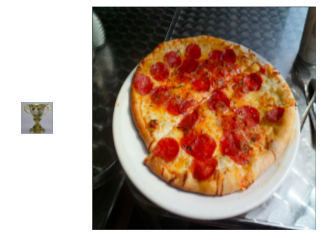
\includegraphics[width=1\textwidth]{recursos/imagens/results/dataset_diff.png}

    Fonte: do próprio autor.
\end{figure}

Adicionalmente, é relevante mencionar que, em amostras pequenas como as do conjunto de dados CIFAR 100, a quantidade de informação a ser preservada é mínima. Isso pode explicar o desempenho inferior do método BPCAPooling, embora não tenha representado uma barreira significativa para os métodos de \textit{pooling} tradicionais, tais como \textit{Max Pooling} e \textit{Avg Pooling}, uma vez que a preservação da espacialidade das amostras de entrada não é a principal preocupação desses métodos.

Além disso, conforme discutido na Seção \ref{results:class}, ao analisar o processo de \textit{fine-tuning} utilizando o método BPCAPooling, destaca-se um comportamento notável no quarto bloco convolucional, onde ocorre uma tendência ascendente na acurácia e uma tendência de redução no \textit{loss} ao longo das épocas de treinamento e validação. Essa tendência sugere que características espaciais importantes provavelmente estão sendo capturadas e retidas no quarto bloco convolucional. É notável que o modelo não apresenta sinais de \textit{overfitting} nesse bloco, indicando que mais épocas poderiam ser empregadas nessa etapa do processo para explorar melhor essa tendência ascendente. Contudo, é crucial considerar que a condução de épocas adicionais demandaria recursos computacionais significativos, devido à complexidade do método e ao custo computacional associado.

A representação da acurácia e \textit{loss} para o conjunto de dados CIFAR 100 está ilustrada nas Figuras \ref{results:fig:datasets:1} e \ref{results:fig:datasets:2}, respectivamente, enquanto as Figuras \ref{results:fig:datasets:3} e \ref{results:fig:datasets:4} mostram a evolução da acurácia e \textit{loss} para o conjunto de dados \textit{Food}-101, todas referentes ao uso do método BPCAPooling.


\begin{figure}[H]
    \centering
    \caption{Evolução de Acurácia no conjunto de dados CIFAR 100.}
    \label{results:fig:datasets:1}
     \begin{subfigure}[t]{0.45\textwidth}
         \centering
         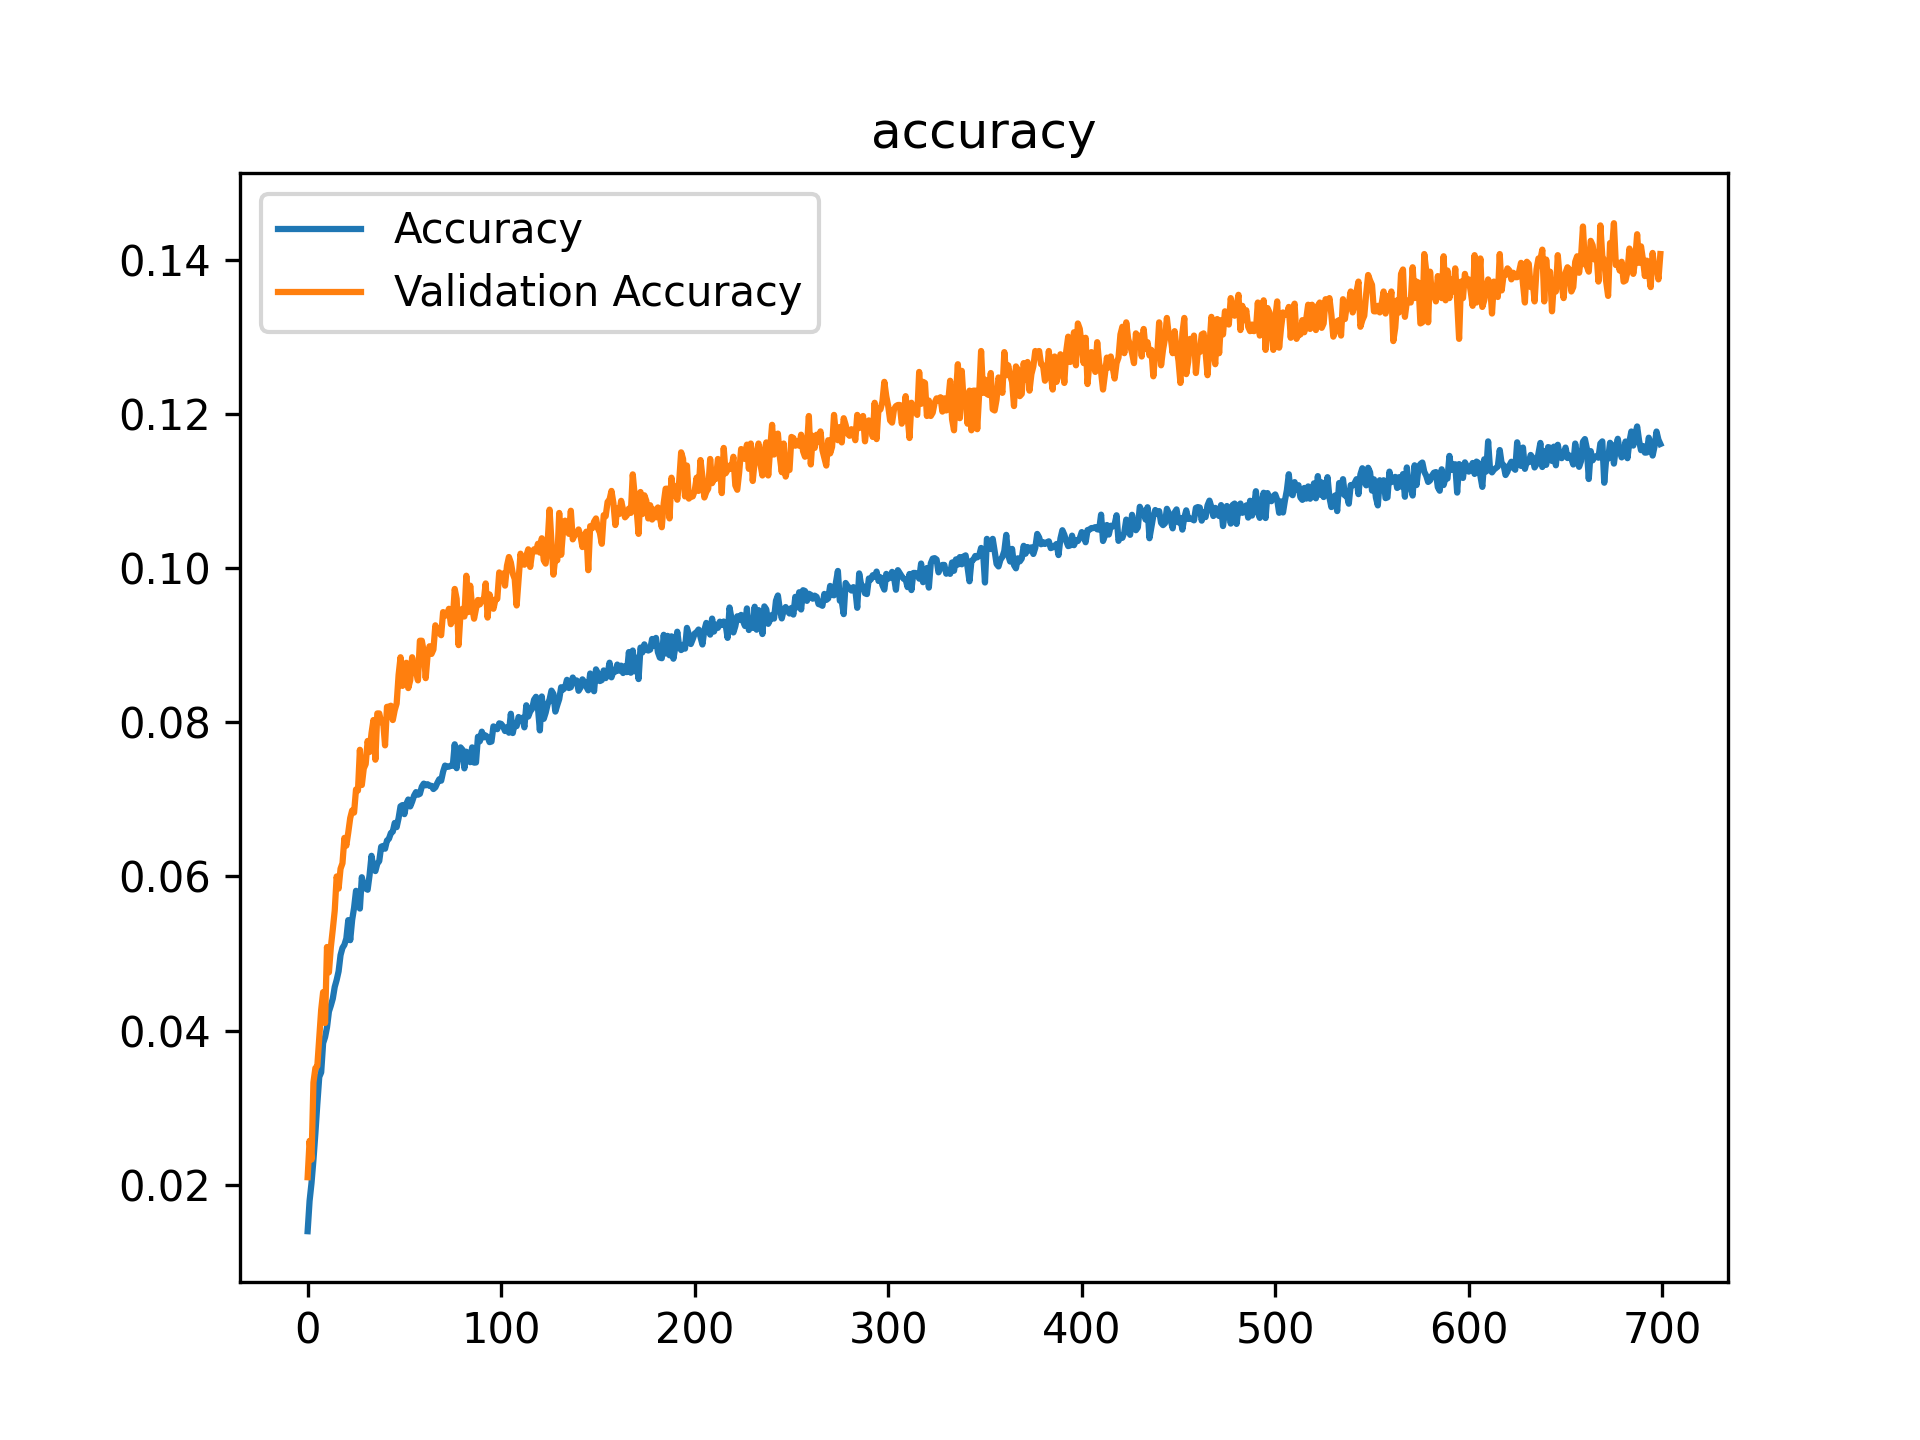
\includegraphics[width=1\linewidth]{recursos/imagens/results/cifar_wp_accuracy.png}
         \caption{Aquecimento.}
         \label{results:fig:datasets:1.1}
     \end{subfigure}%
     ~ 
     \begin{subfigure}[t]{0.45\textwidth}
         \centering
         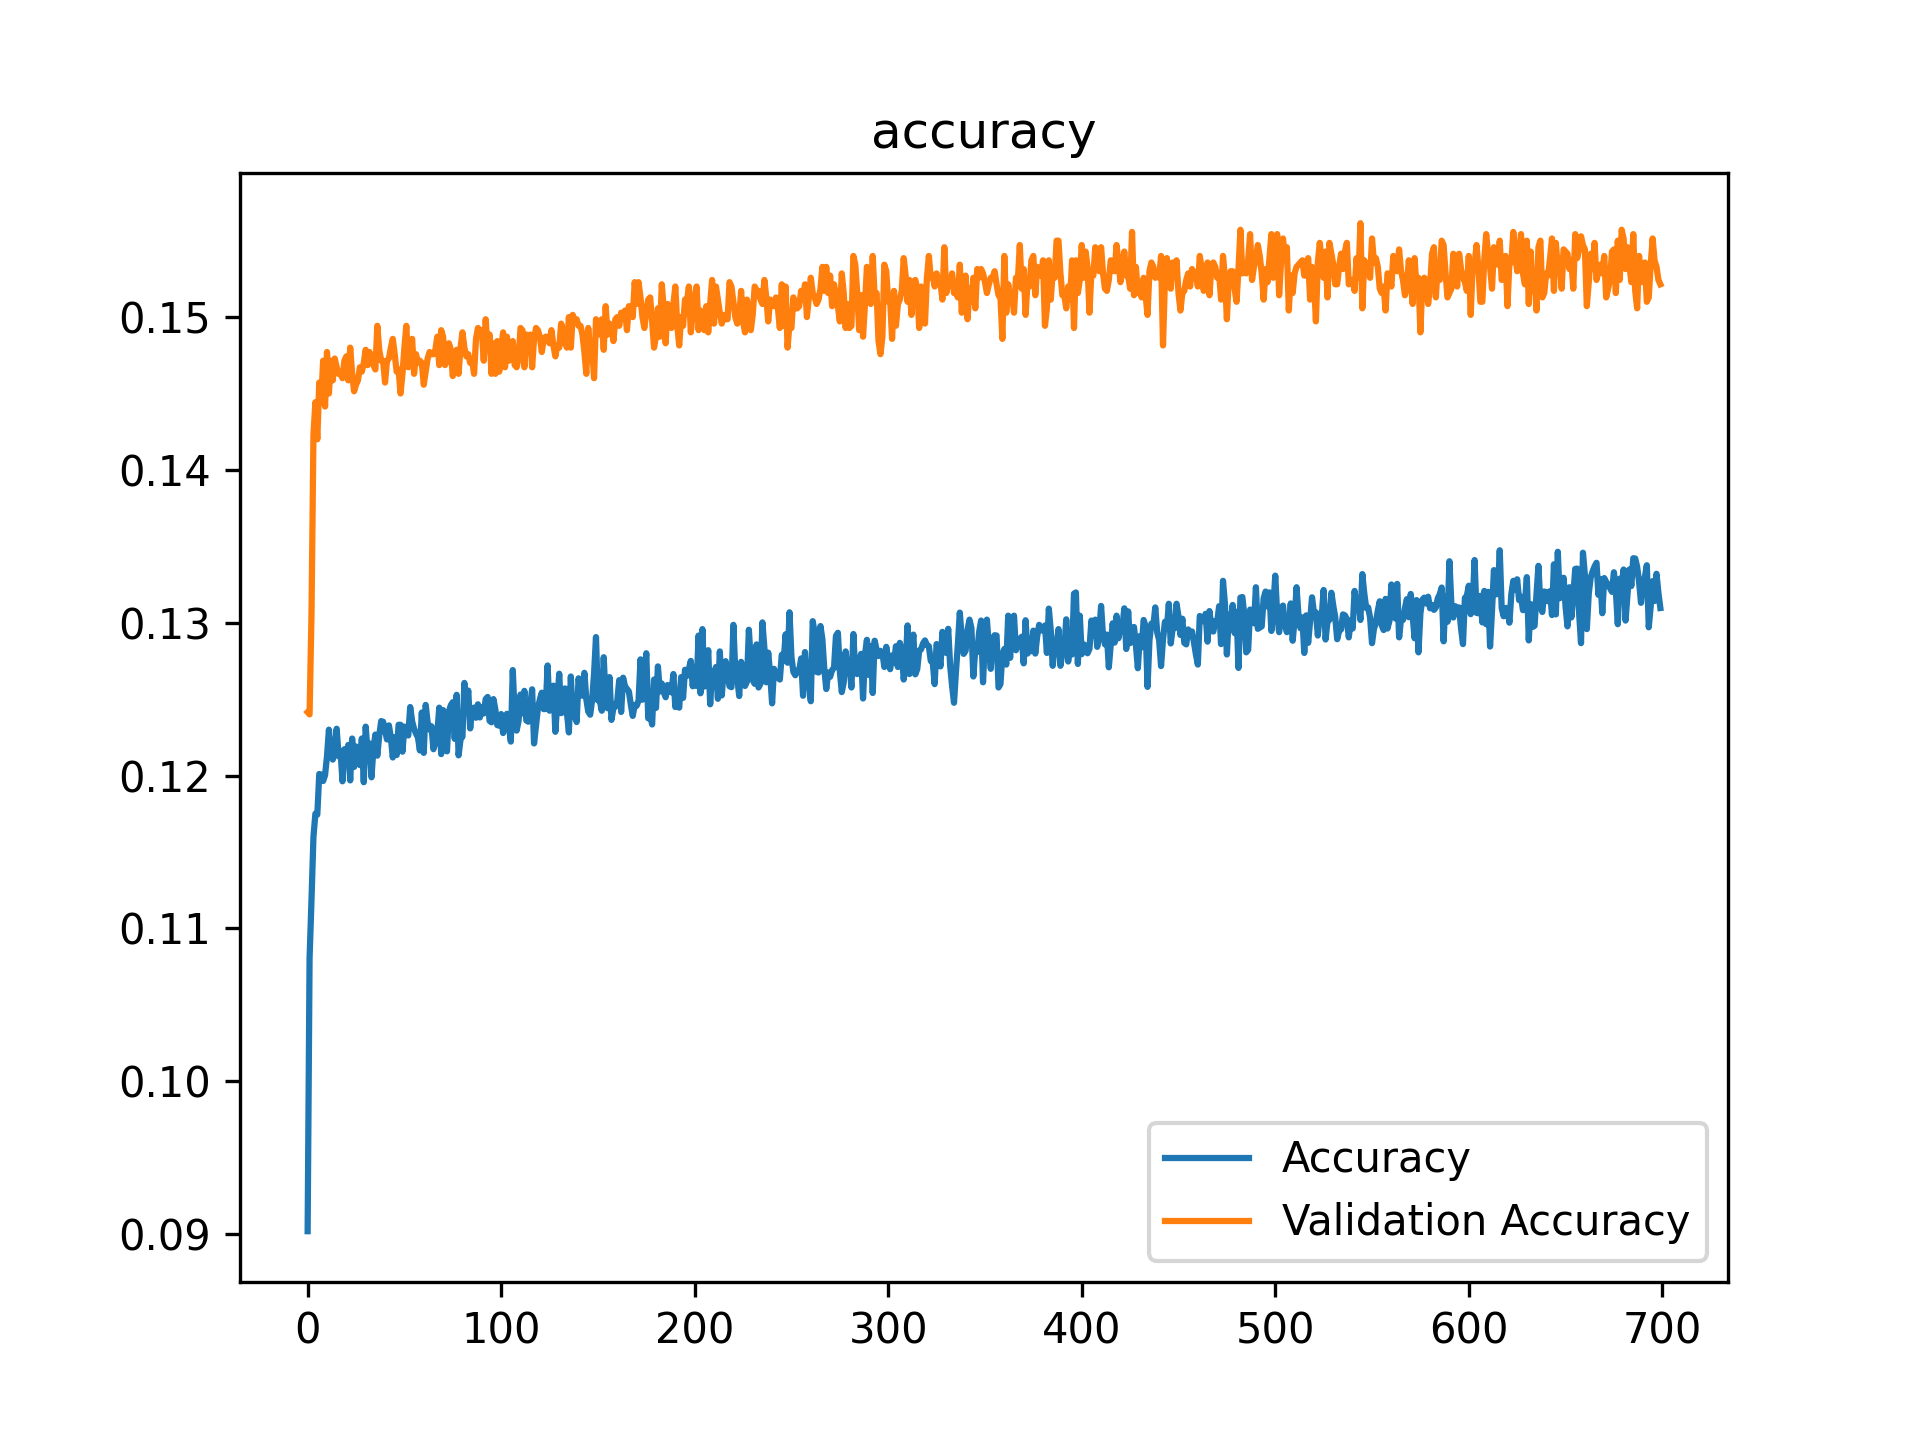
\includegraphics[width=1\linewidth]{recursos/imagens/results/cifar_accuracy1.png}
         \caption{Bloco 5.}
         \label{results:fig:datasets:1.2}
     \end{subfigure}%
     ~ 
     
     \begin{subfigure}[t]{0.45\textwidth}
         \centering
         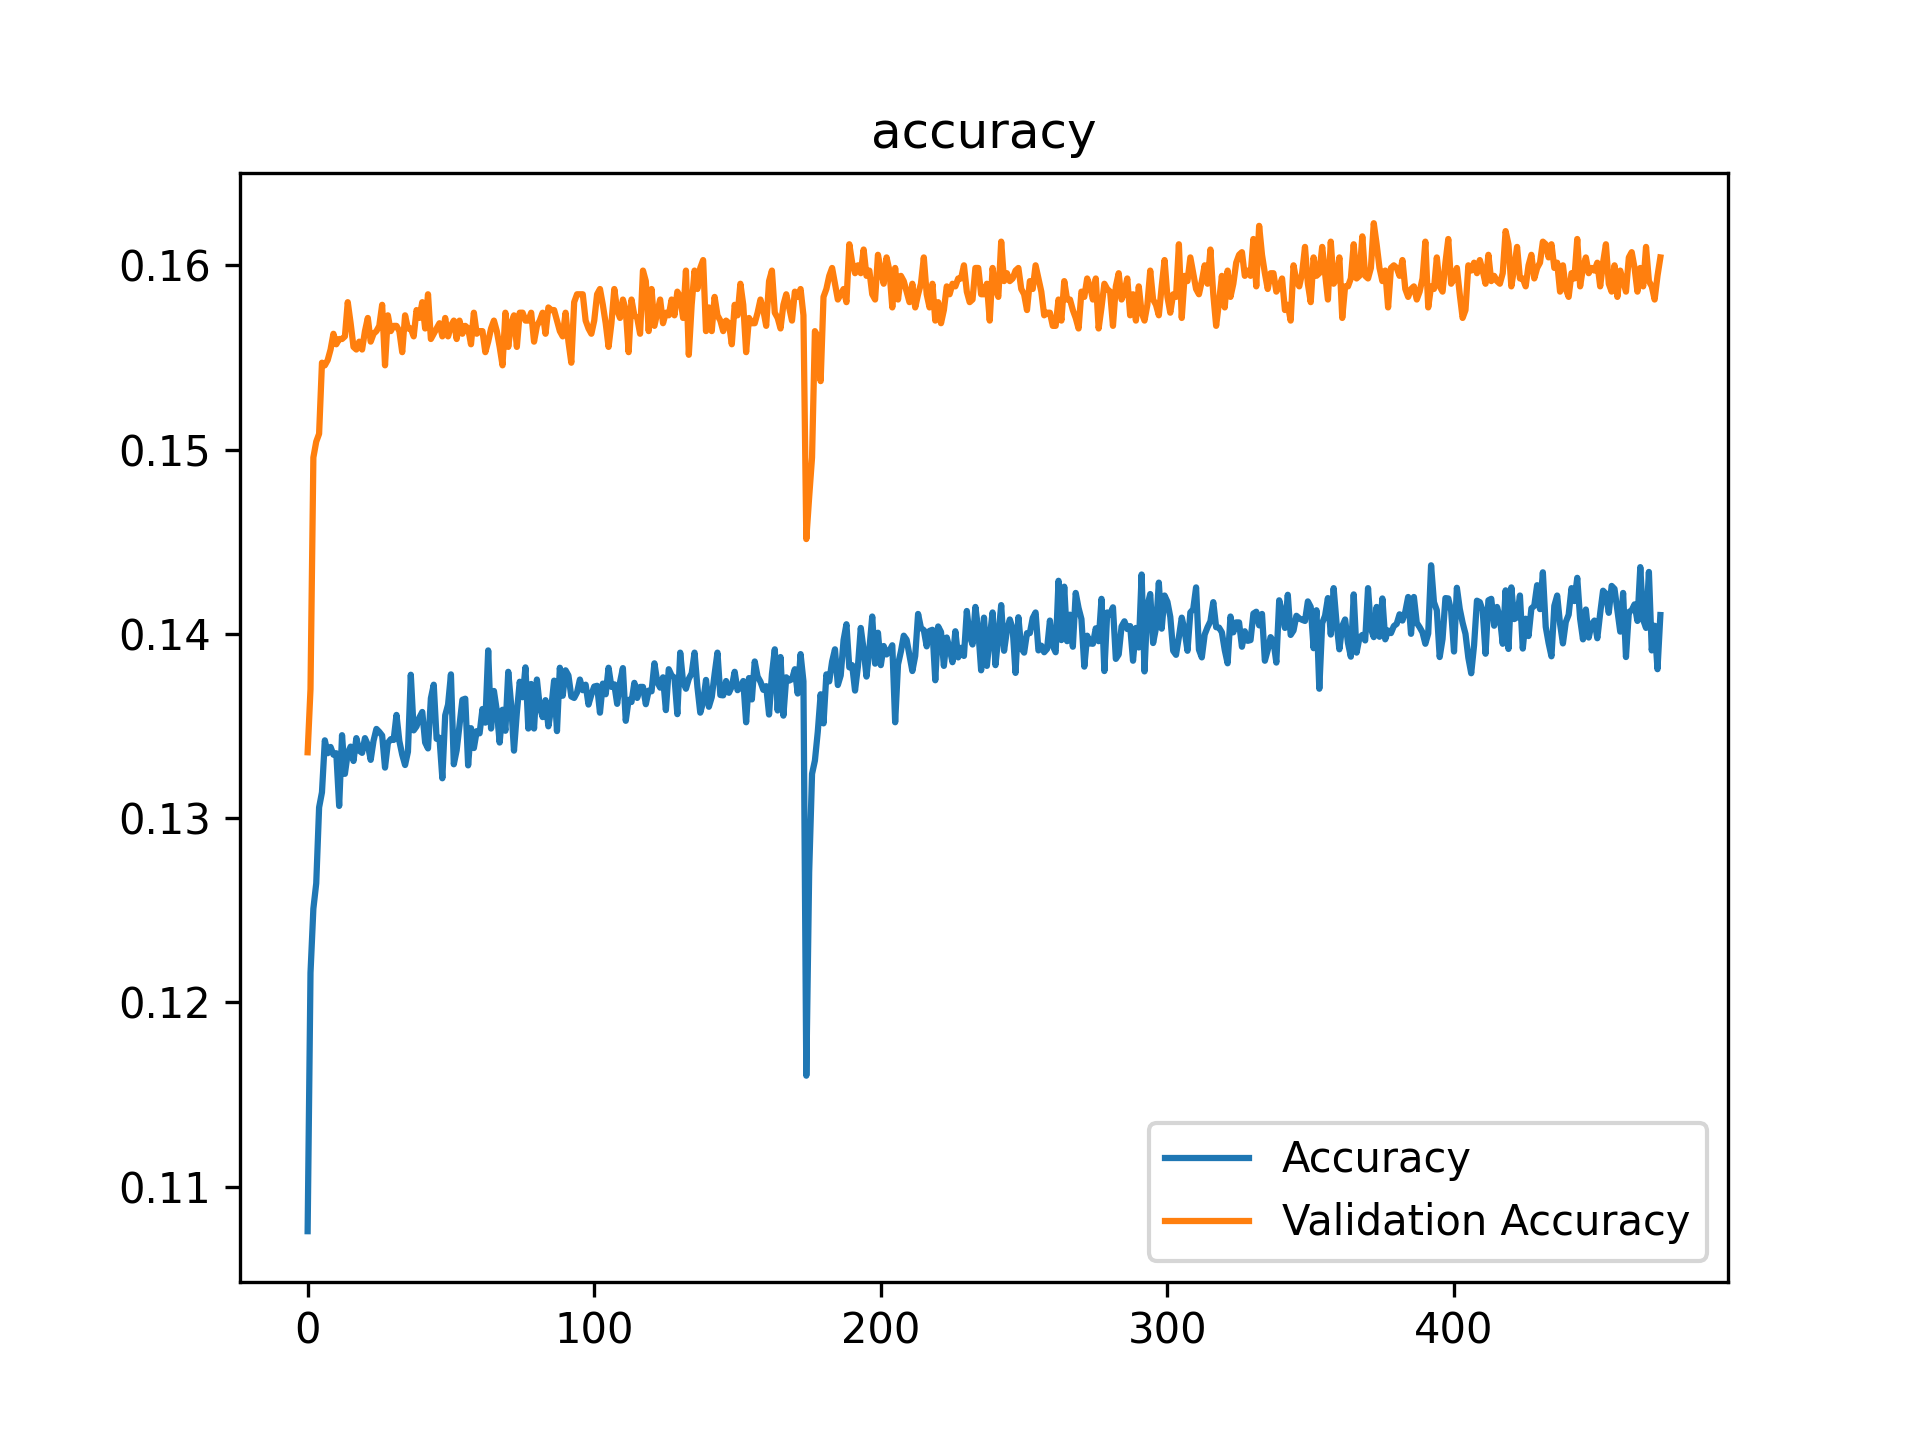
\includegraphics[width=1\linewidth]{recursos/imagens/results/cifar_accuracy2.png}
         \caption{Bloco 4.}
         \label{results:fig:datasets:1.3}
     \end{subfigure}
     ~
     \begin{subfigure}[t]{0.45\textwidth}
         \centering
         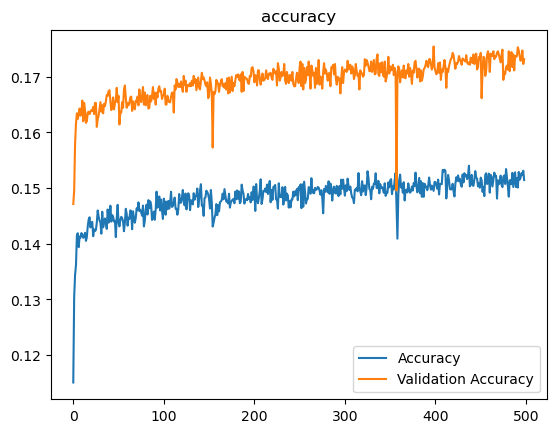
\includegraphics[width=1\linewidth]{recursos/imagens/results/cifar_accuracy3.png}
         \caption{Bloco 3.}
         \label{results:fig:datasets:1.4}
     \end{subfigure}
     
     Fonte: do próprio autor.
 \end{figure}

\begin{figure}[H]
    \centering
    \caption{Evolução de \textit{Loss} no conjunto de dados CIFAR 100.}
    \label{results:fig:datasets:2}
     \begin{subfigure}[t]{0.45\textwidth}
         \centering
         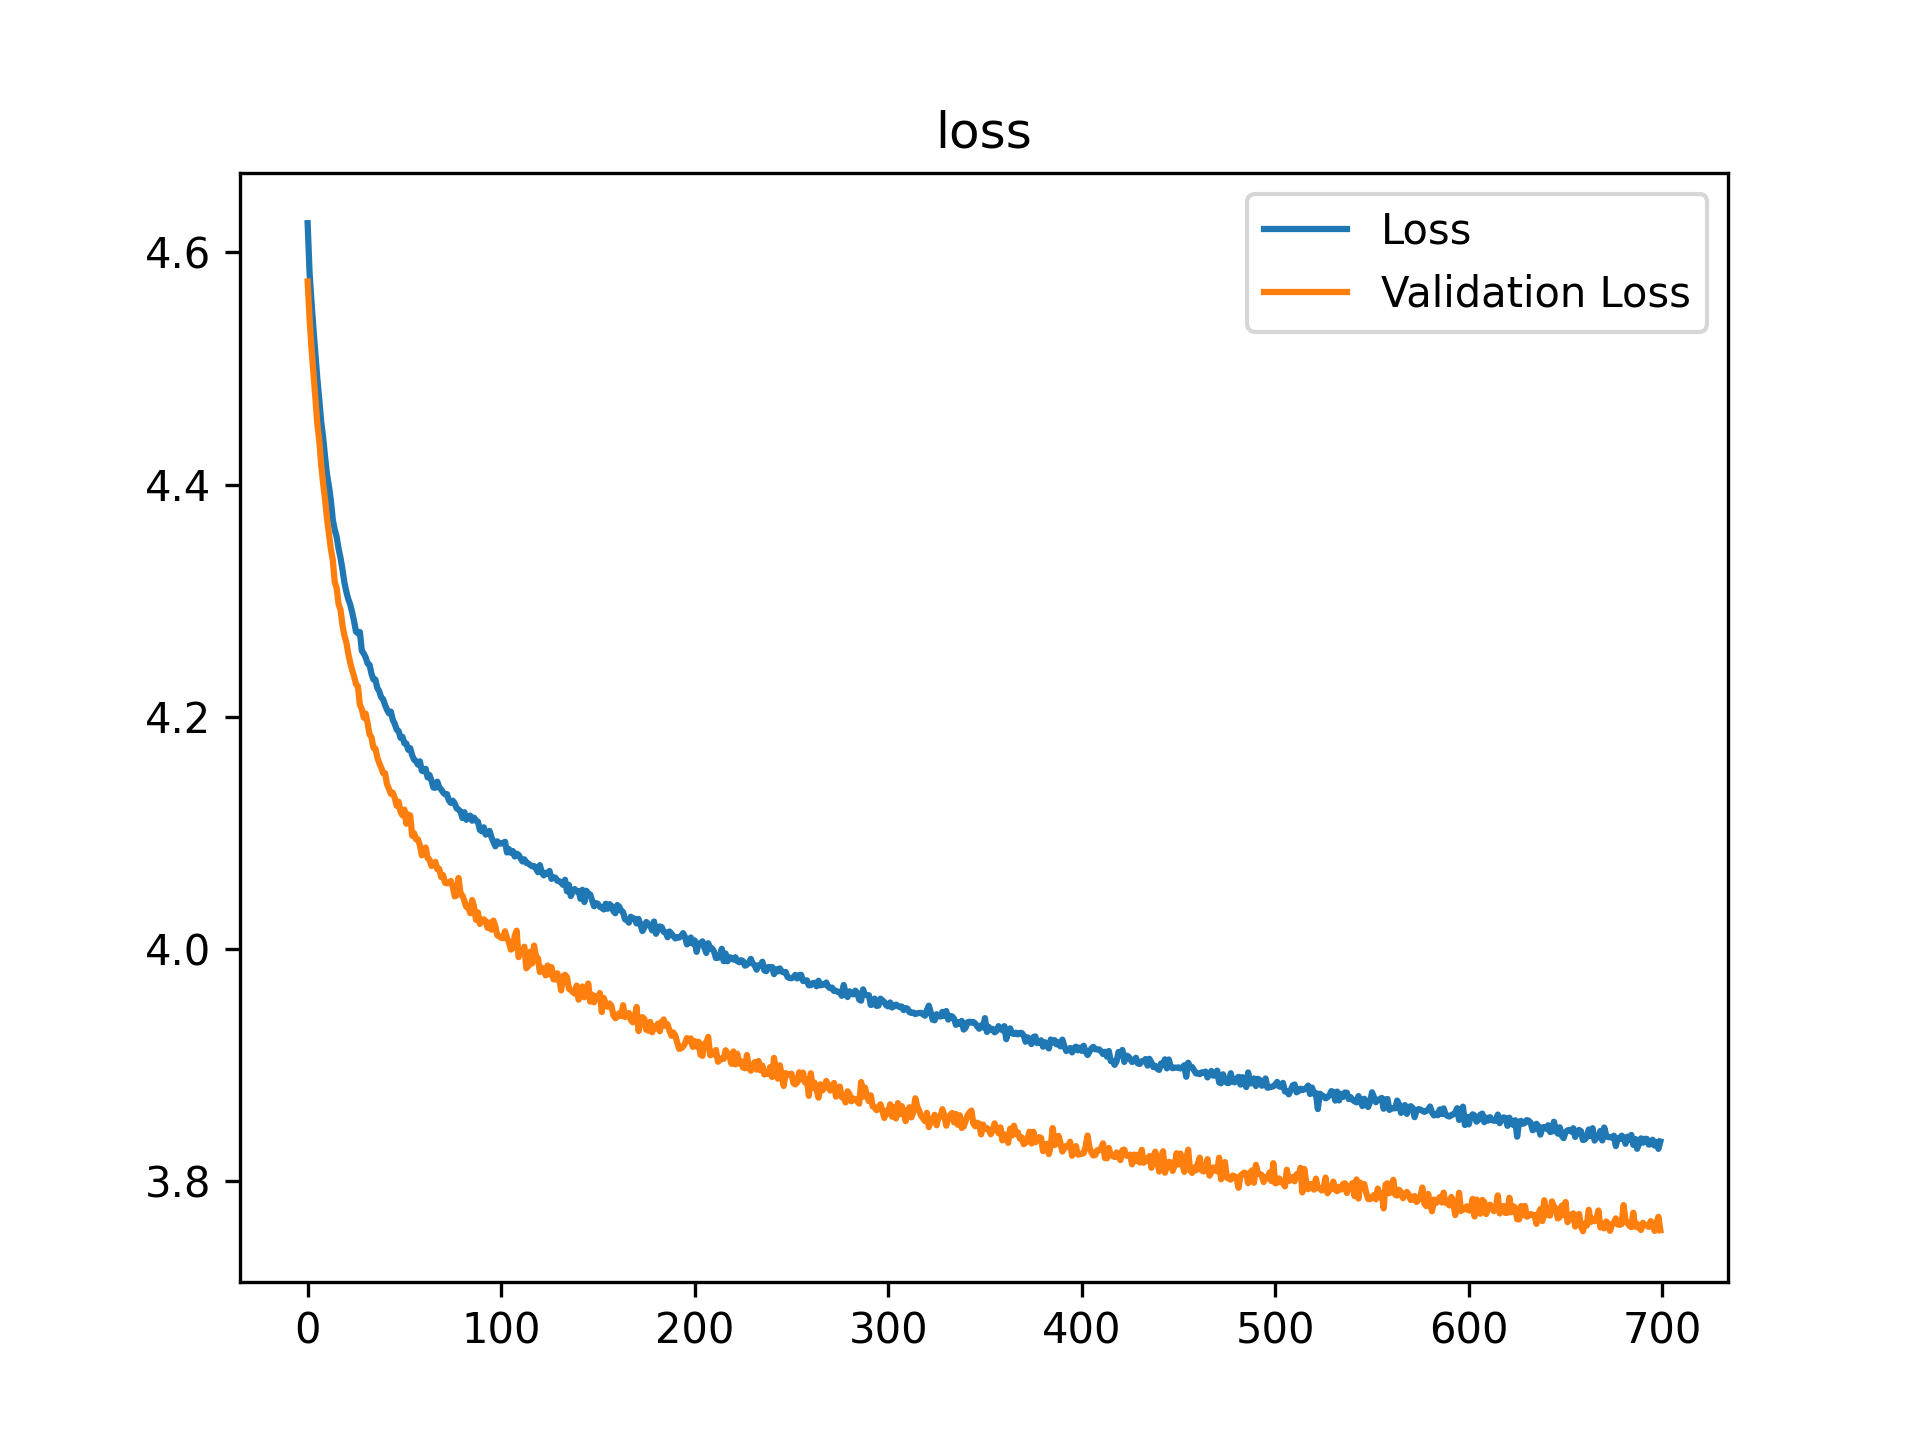
\includegraphics[width=1\linewidth]{recursos/imagens/results/cifar_wp_loss.png}
         \caption{Aquecimento.}
         \label{results:fig:datasets:2.1}
     \end{subfigure}%
     ~ 
     \begin{subfigure}[t]{0.45\textwidth}
         \centering
         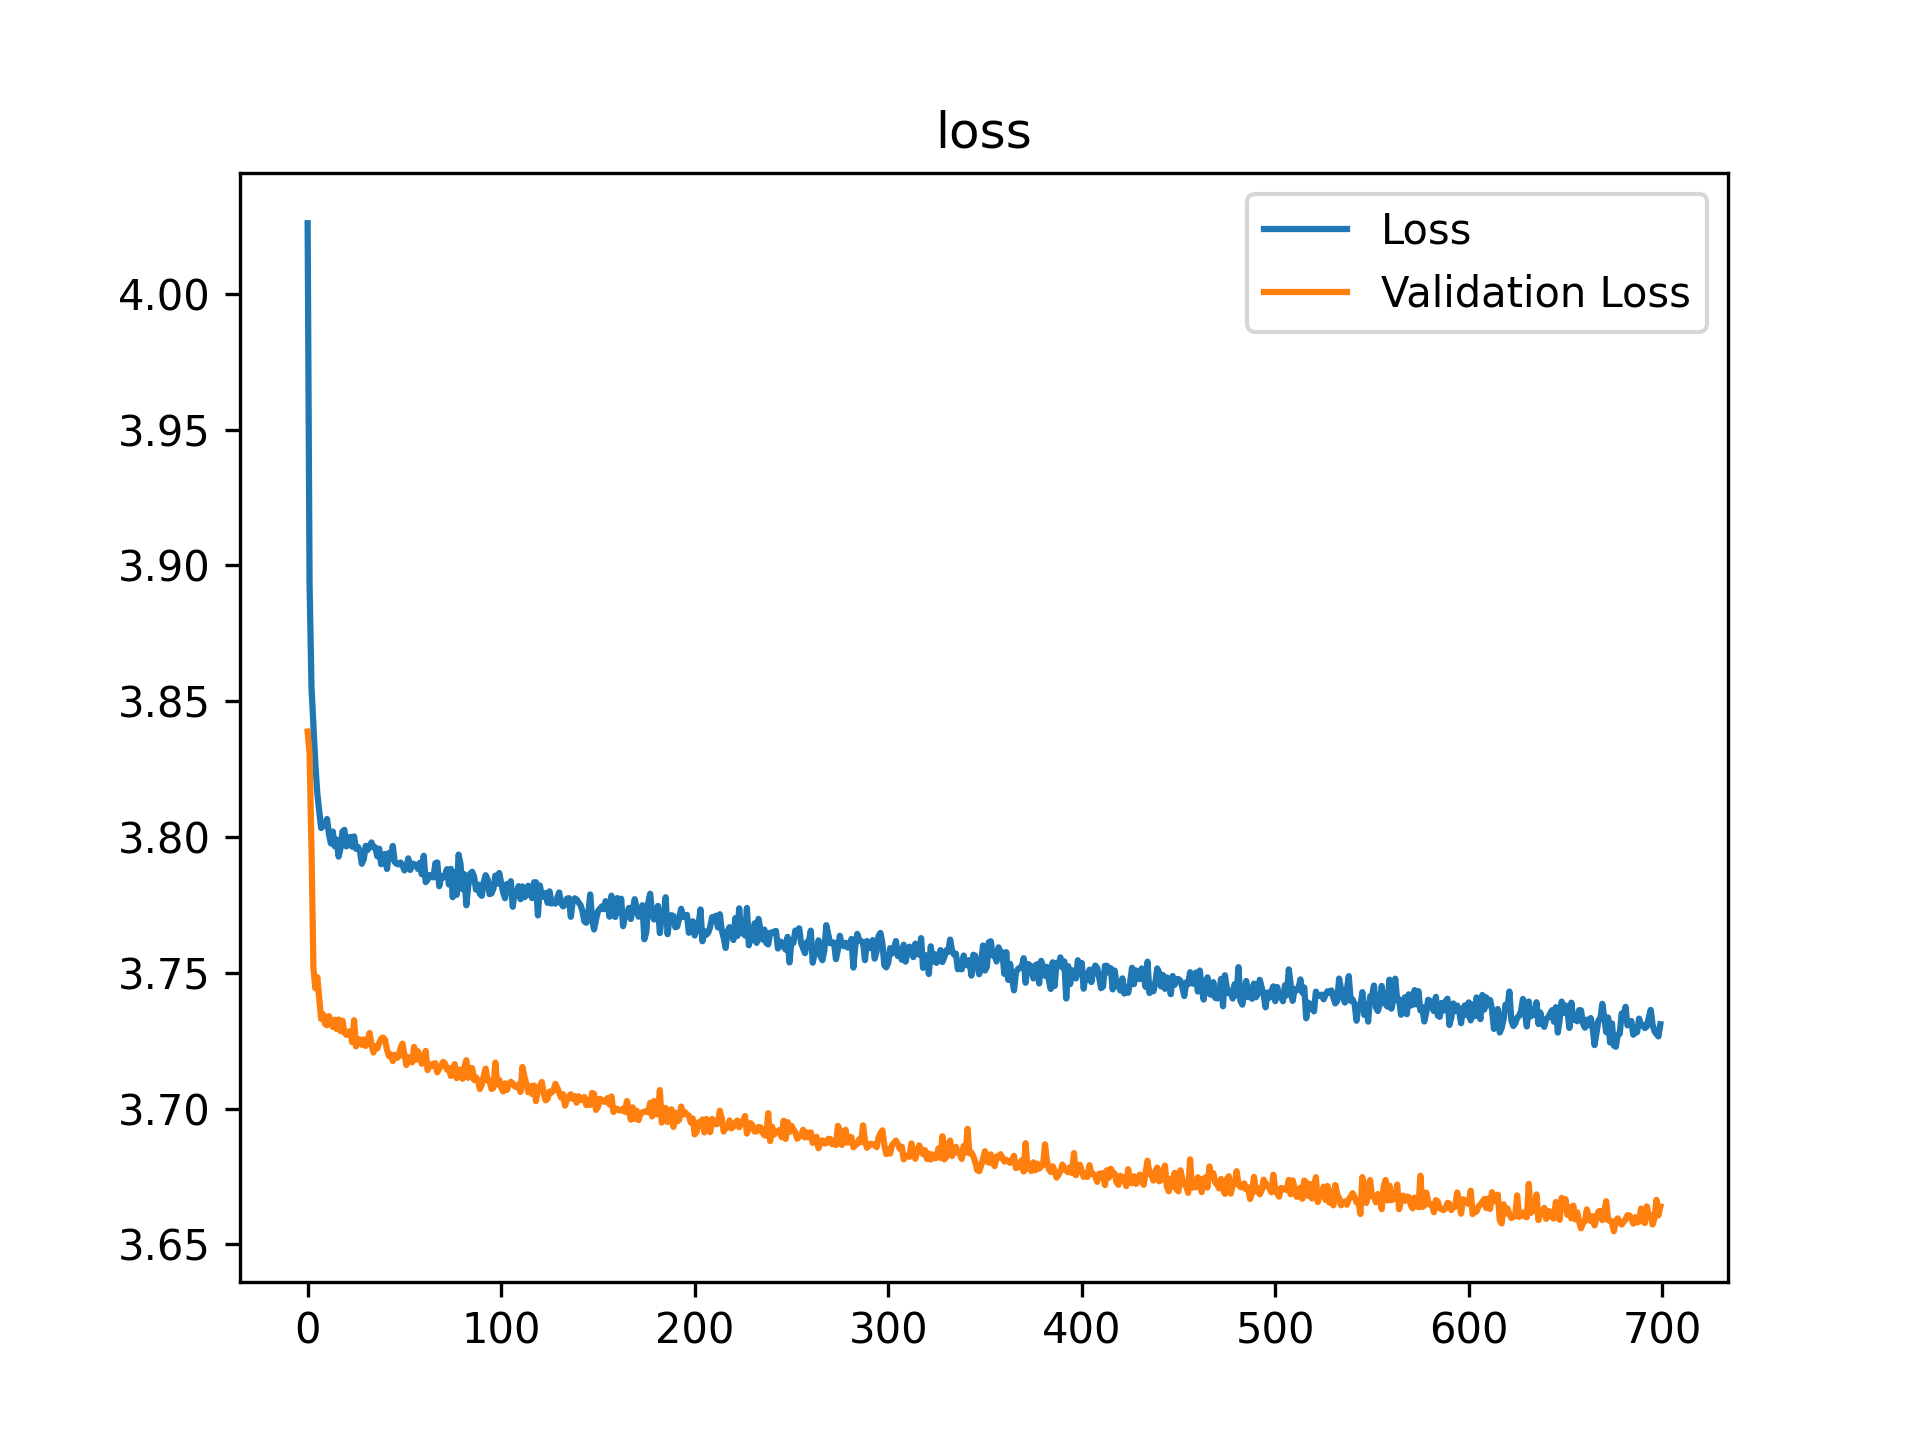
\includegraphics[width=1\linewidth]{recursos/imagens/results/cifar_loss1.png}
         \caption{Bloco 5.}
         \label{results:fig:datasets:2.2}
     \end{subfigure}%
     ~ 
     
     \begin{subfigure}[t]{0.45\textwidth}
         \centering
         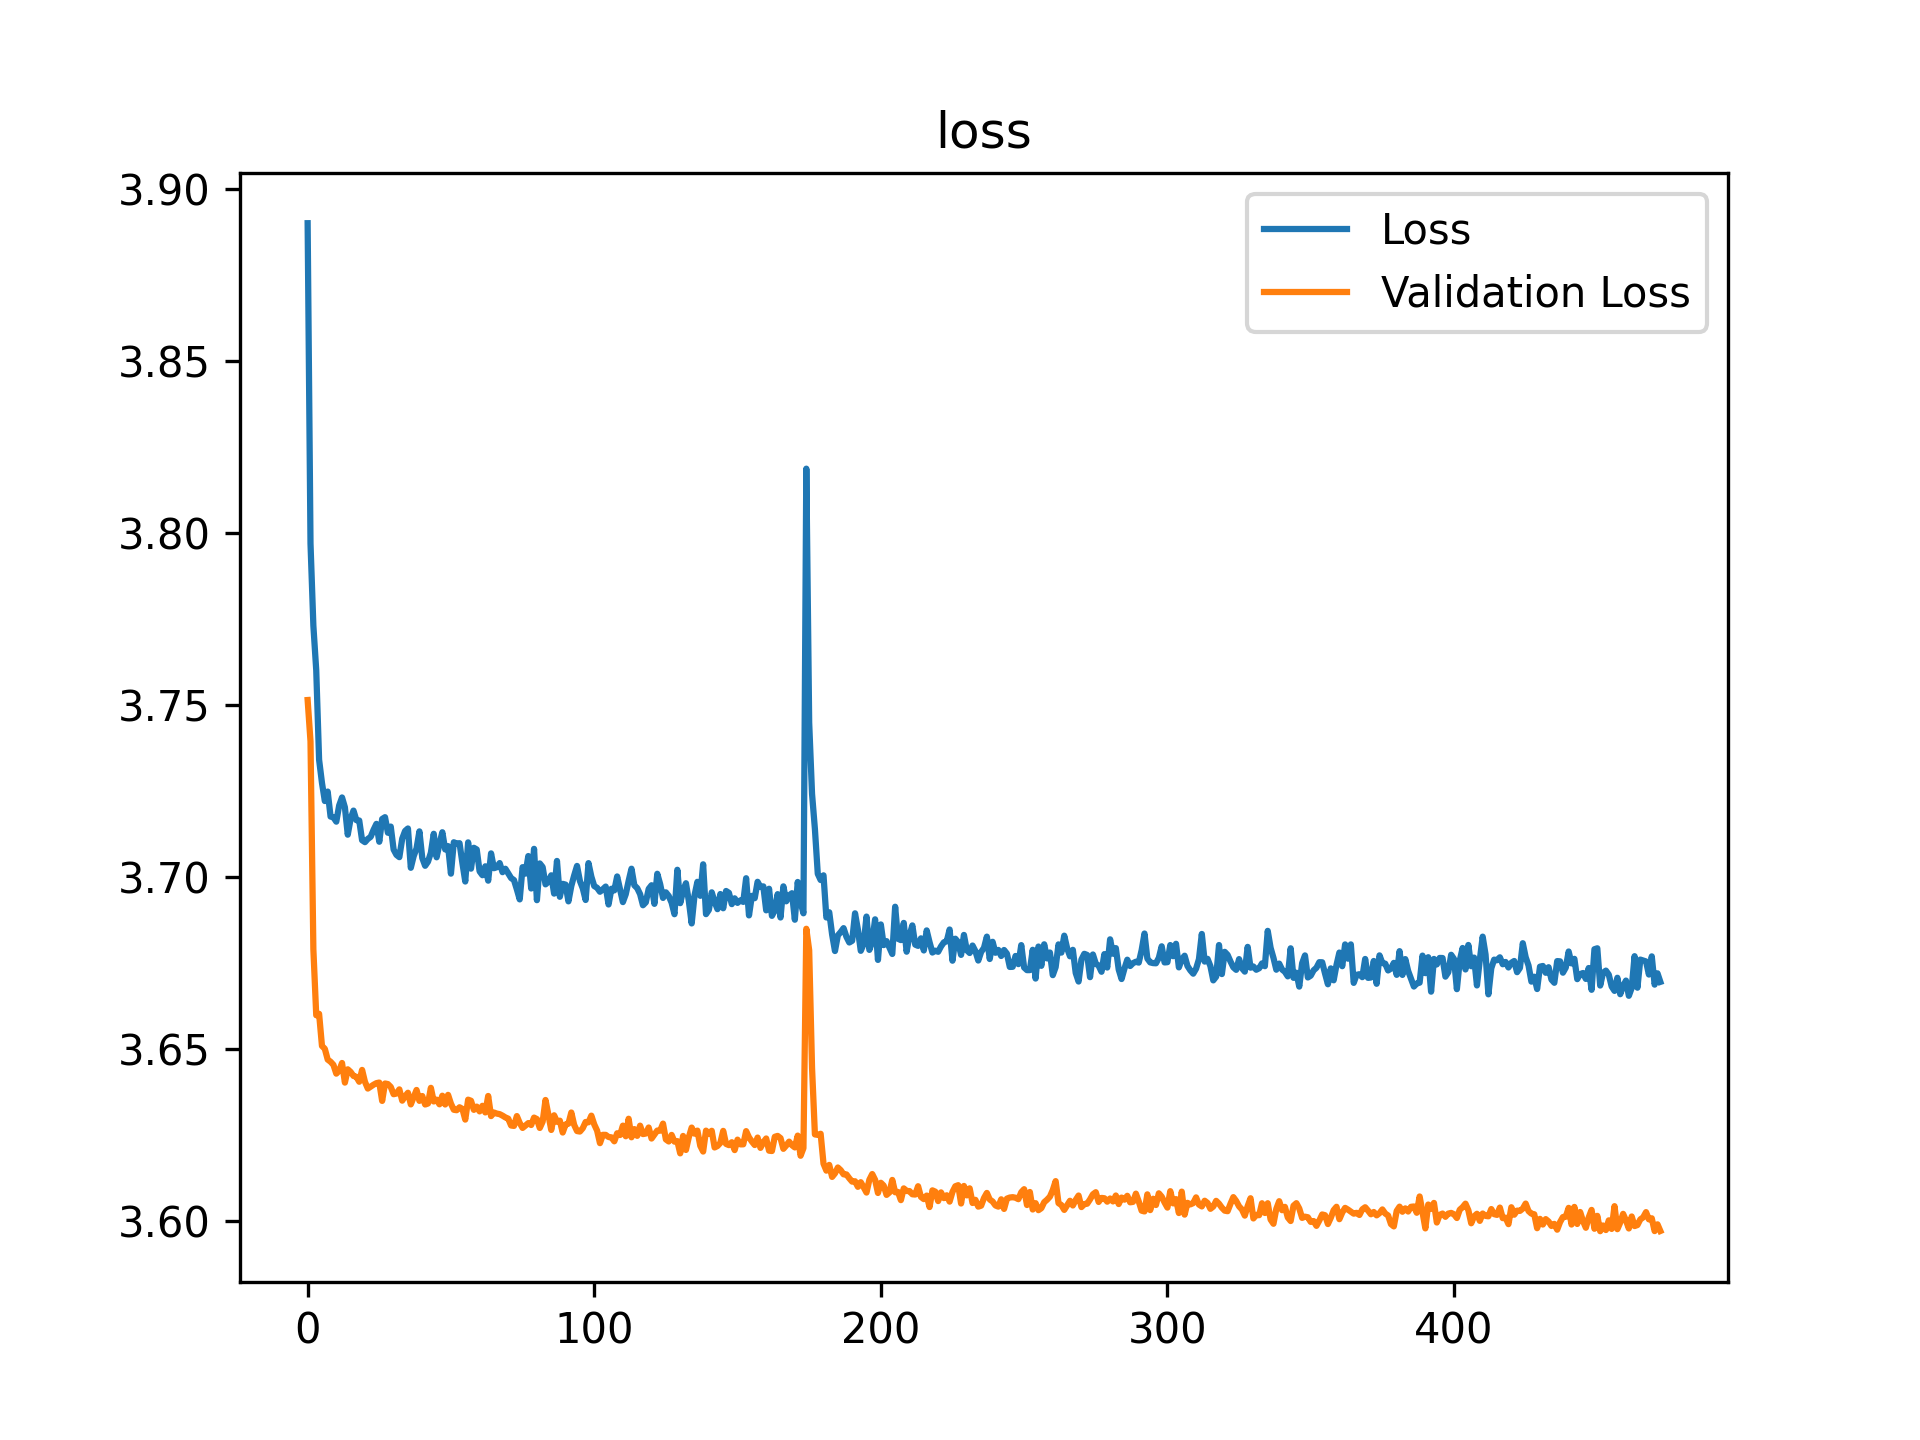
\includegraphics[width=1\linewidth]{recursos/imagens/results/cifar_loss2.png}
         \caption{Bloco 4.}
         \label{results:fig:datasets:2.3}
     \end{subfigure}
     ~
     \begin{subfigure}[t]{0.45\textwidth}
         \centering
         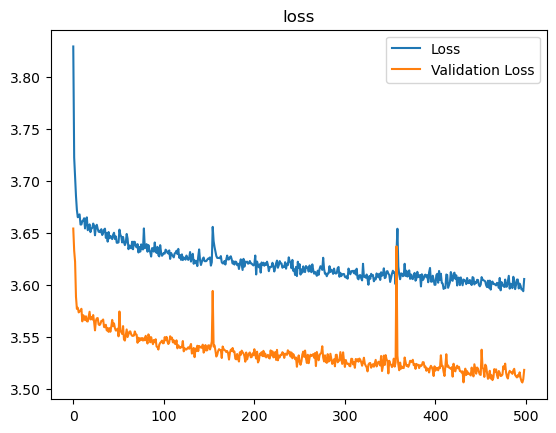
\includegraphics[width=1\linewidth]{recursos/imagens/results/cifar_loss3.png}
         \caption{Bloco 3.}
         \label{results:fig:datasets:2.4}
     \end{subfigure}
     
     Fonte: do próprio autor.
 \end{figure}


\begin{figure}[H]
    \centering
    \caption{Evolução de Acurácia no conjunto de dados \textit{Food}-101.}
    \label{results:fig:datasets:3}
     \begin{subfigure}[t]{0.45\textwidth}
         \centering
         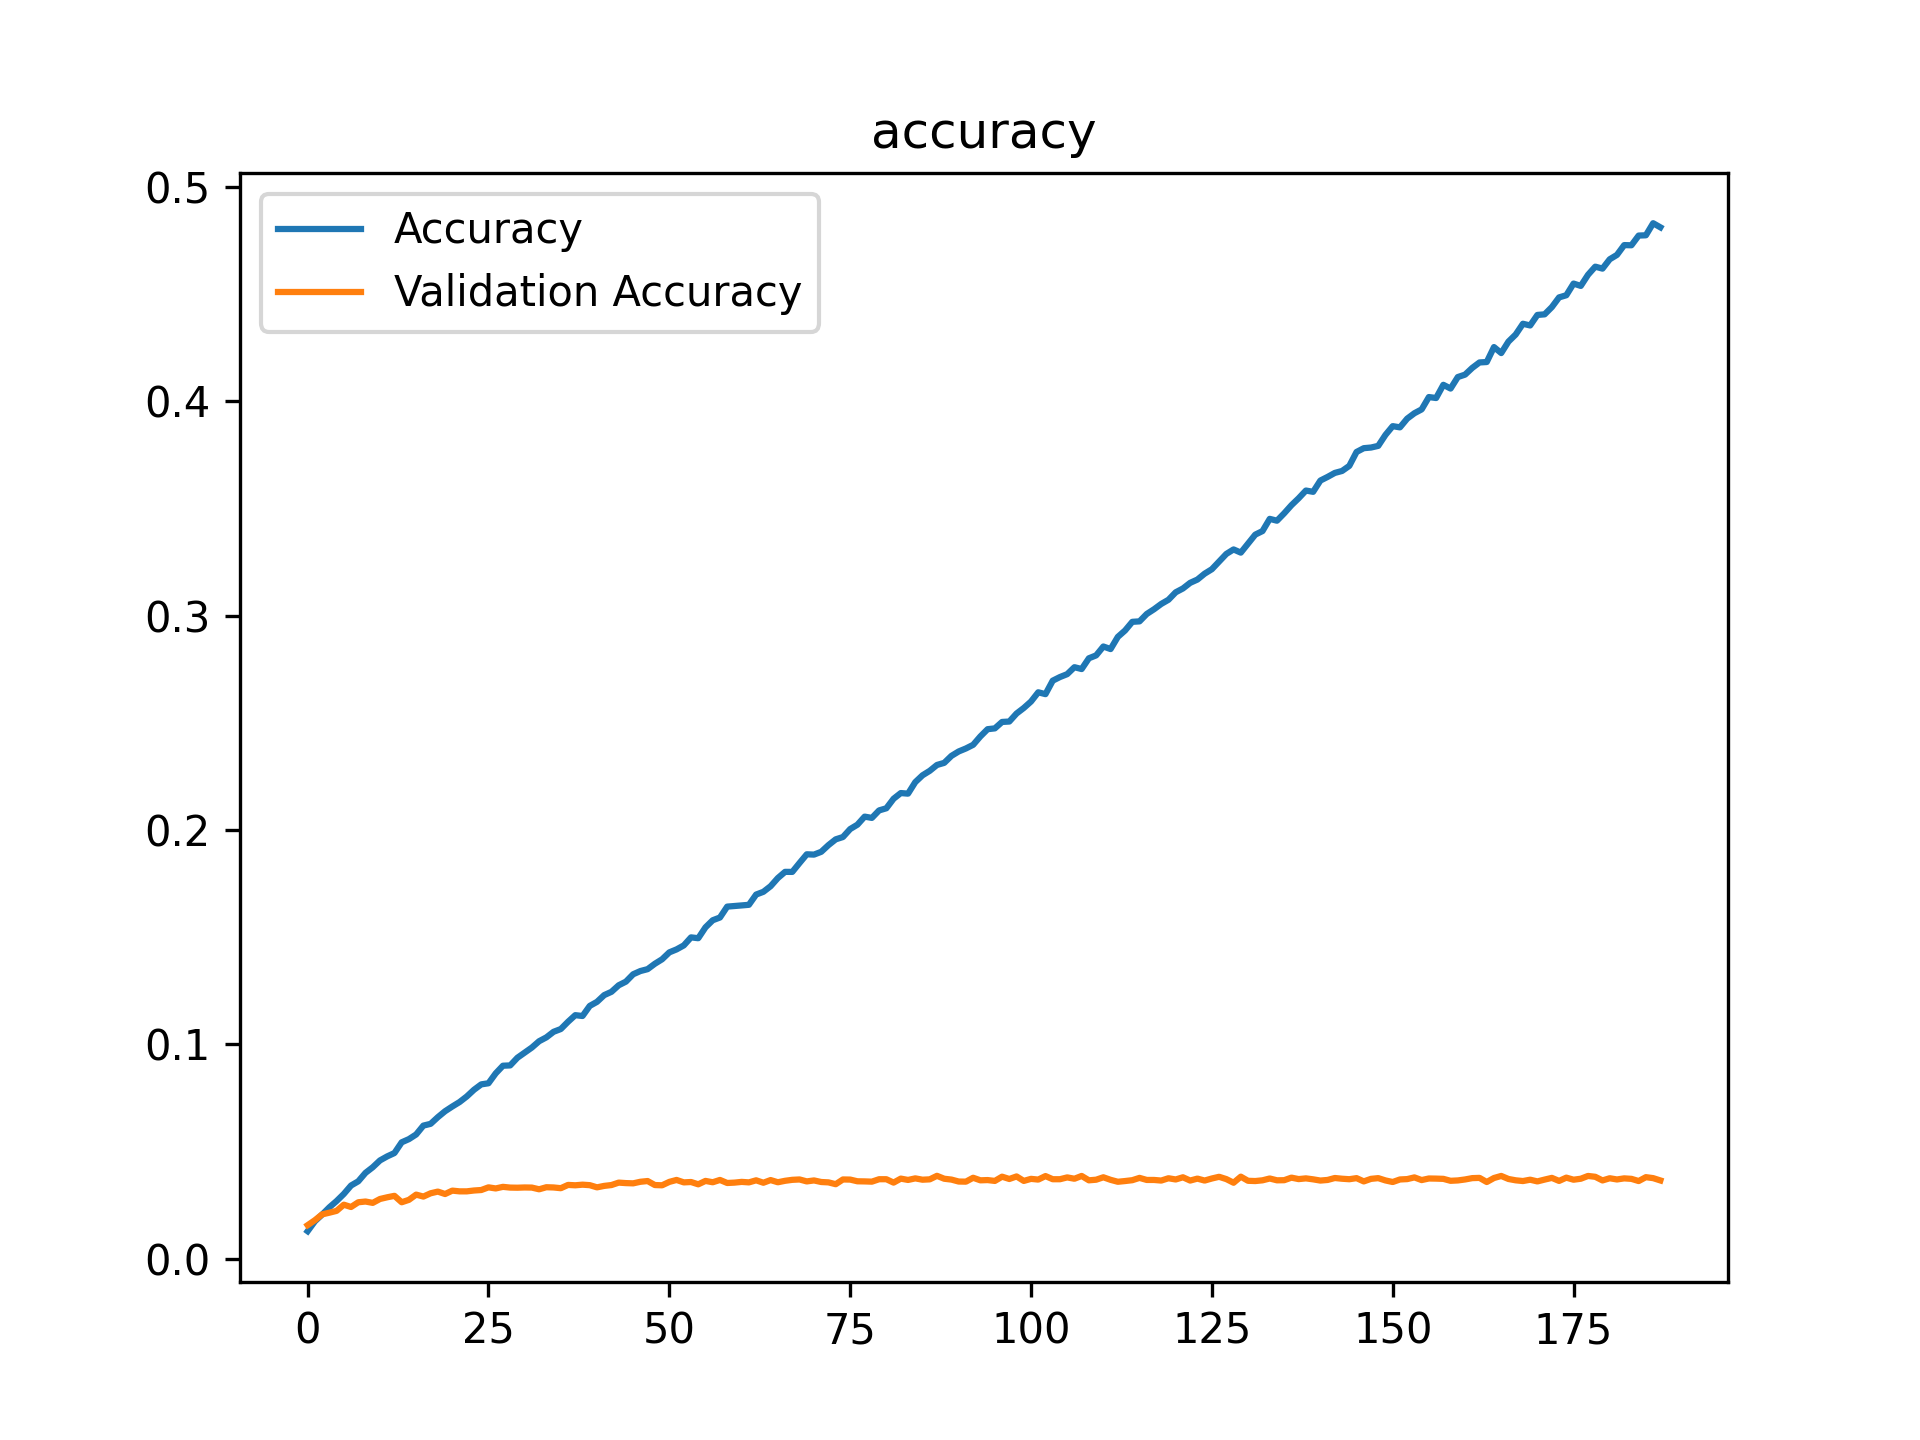
\includegraphics[width=1\linewidth]{recursos/imagens/results/food_wp_accuracy.png}
         \caption{Aquecimento.}
         \label{results:fig:datasets:3.1}
     \end{subfigure}%
     ~ 
     \begin{subfigure}[t]{0.45\textwidth}
         \centering
         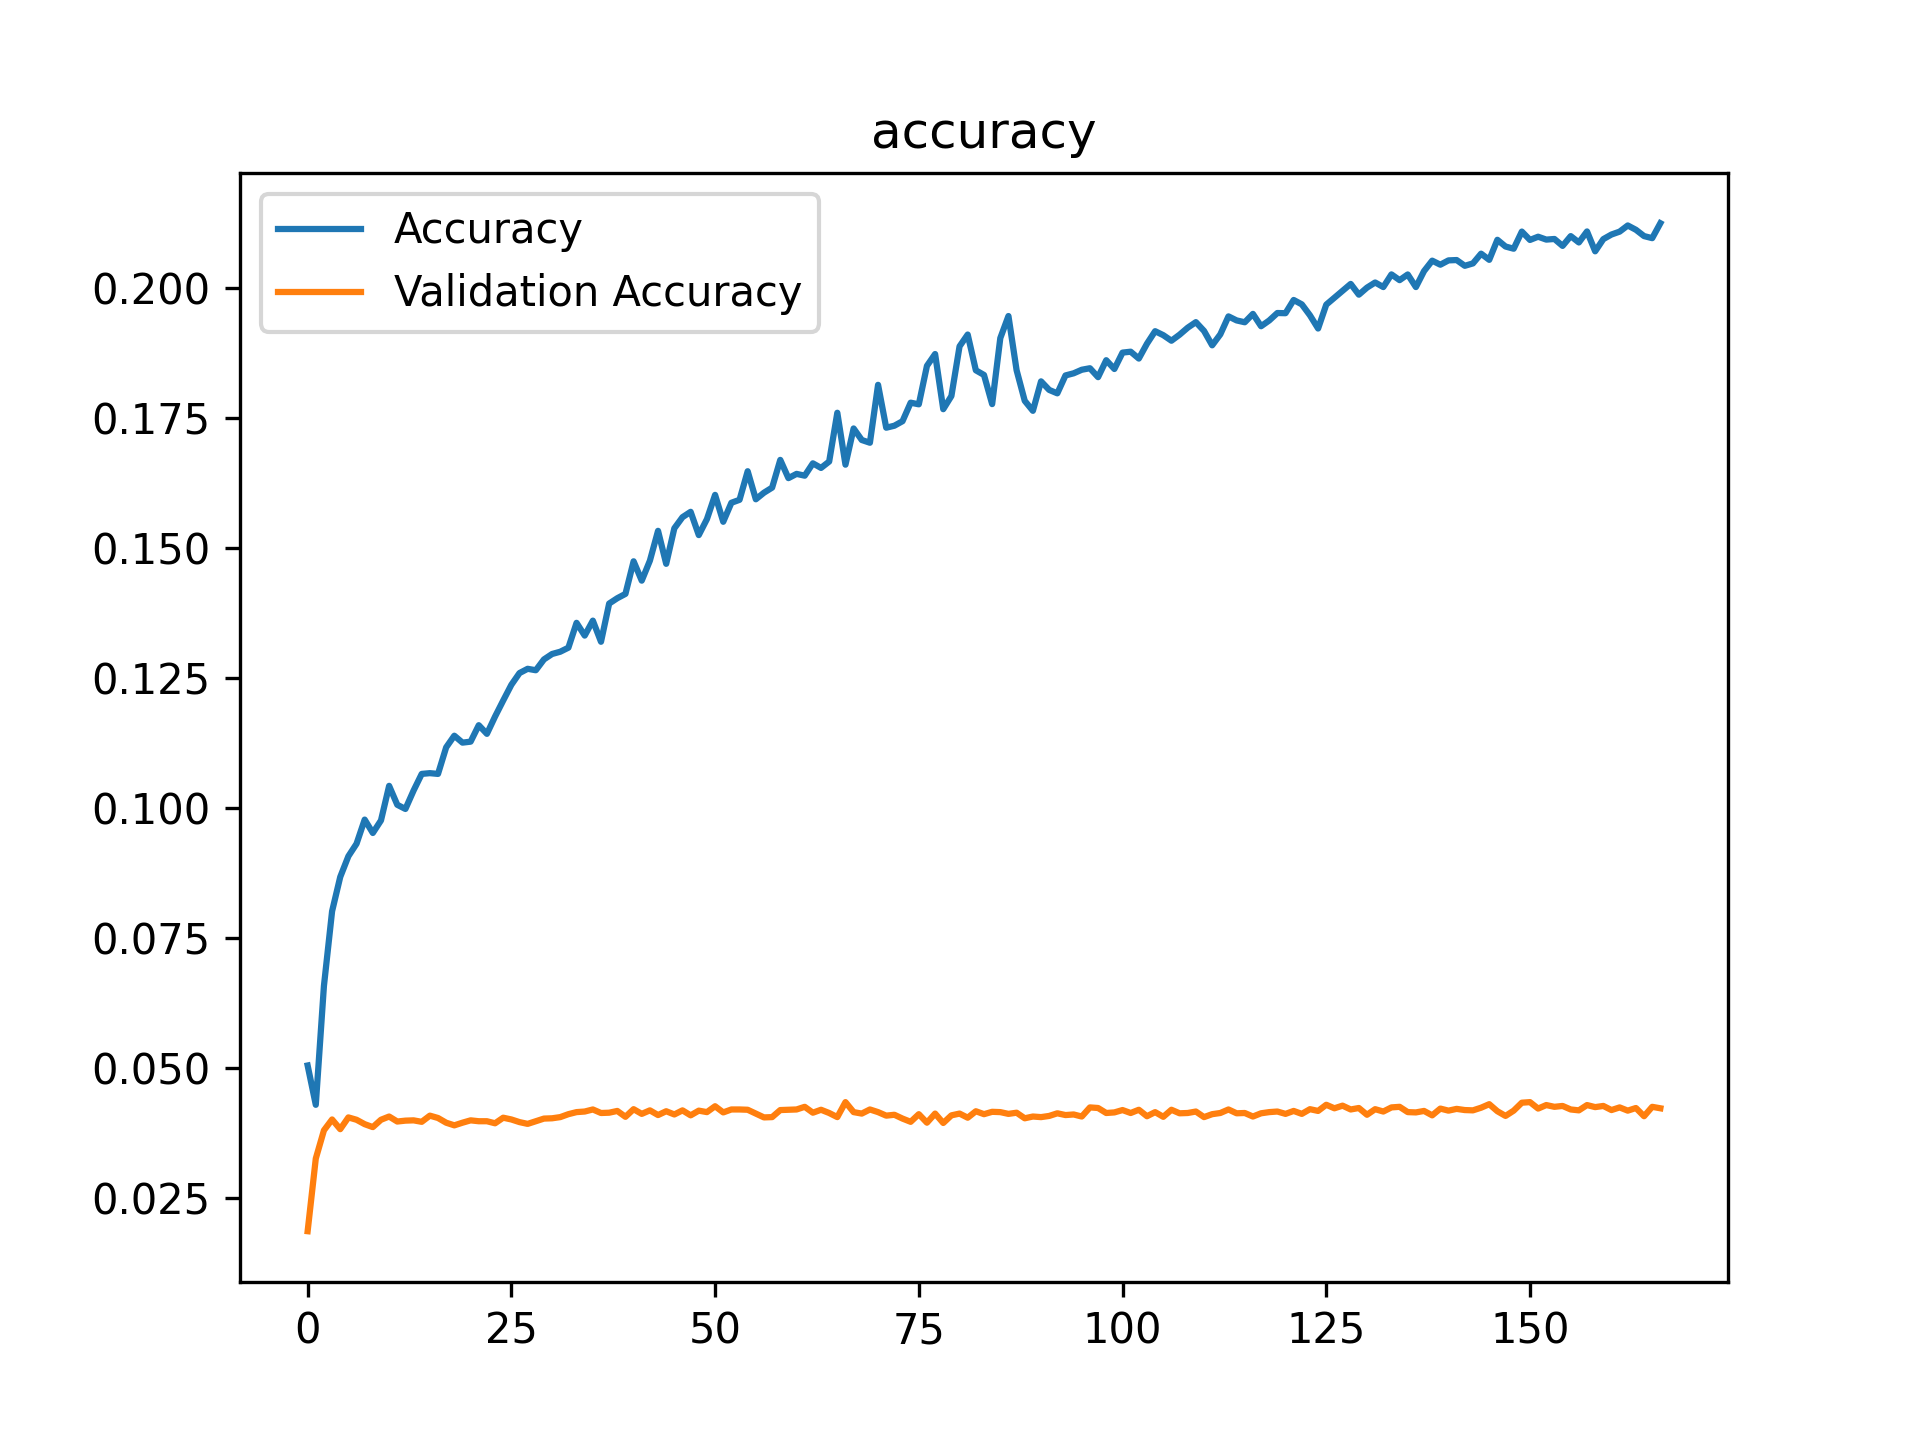
\includegraphics[width=1\linewidth]{recursos/imagens/results/food_accuracy1.png}
         \caption{Bloco 5.}
         \label{results:fig:datasets:3.2}
     \end{subfigure}%
     ~ 
     
     \begin{subfigure}[t]{0.45\textwidth}
         \centering
         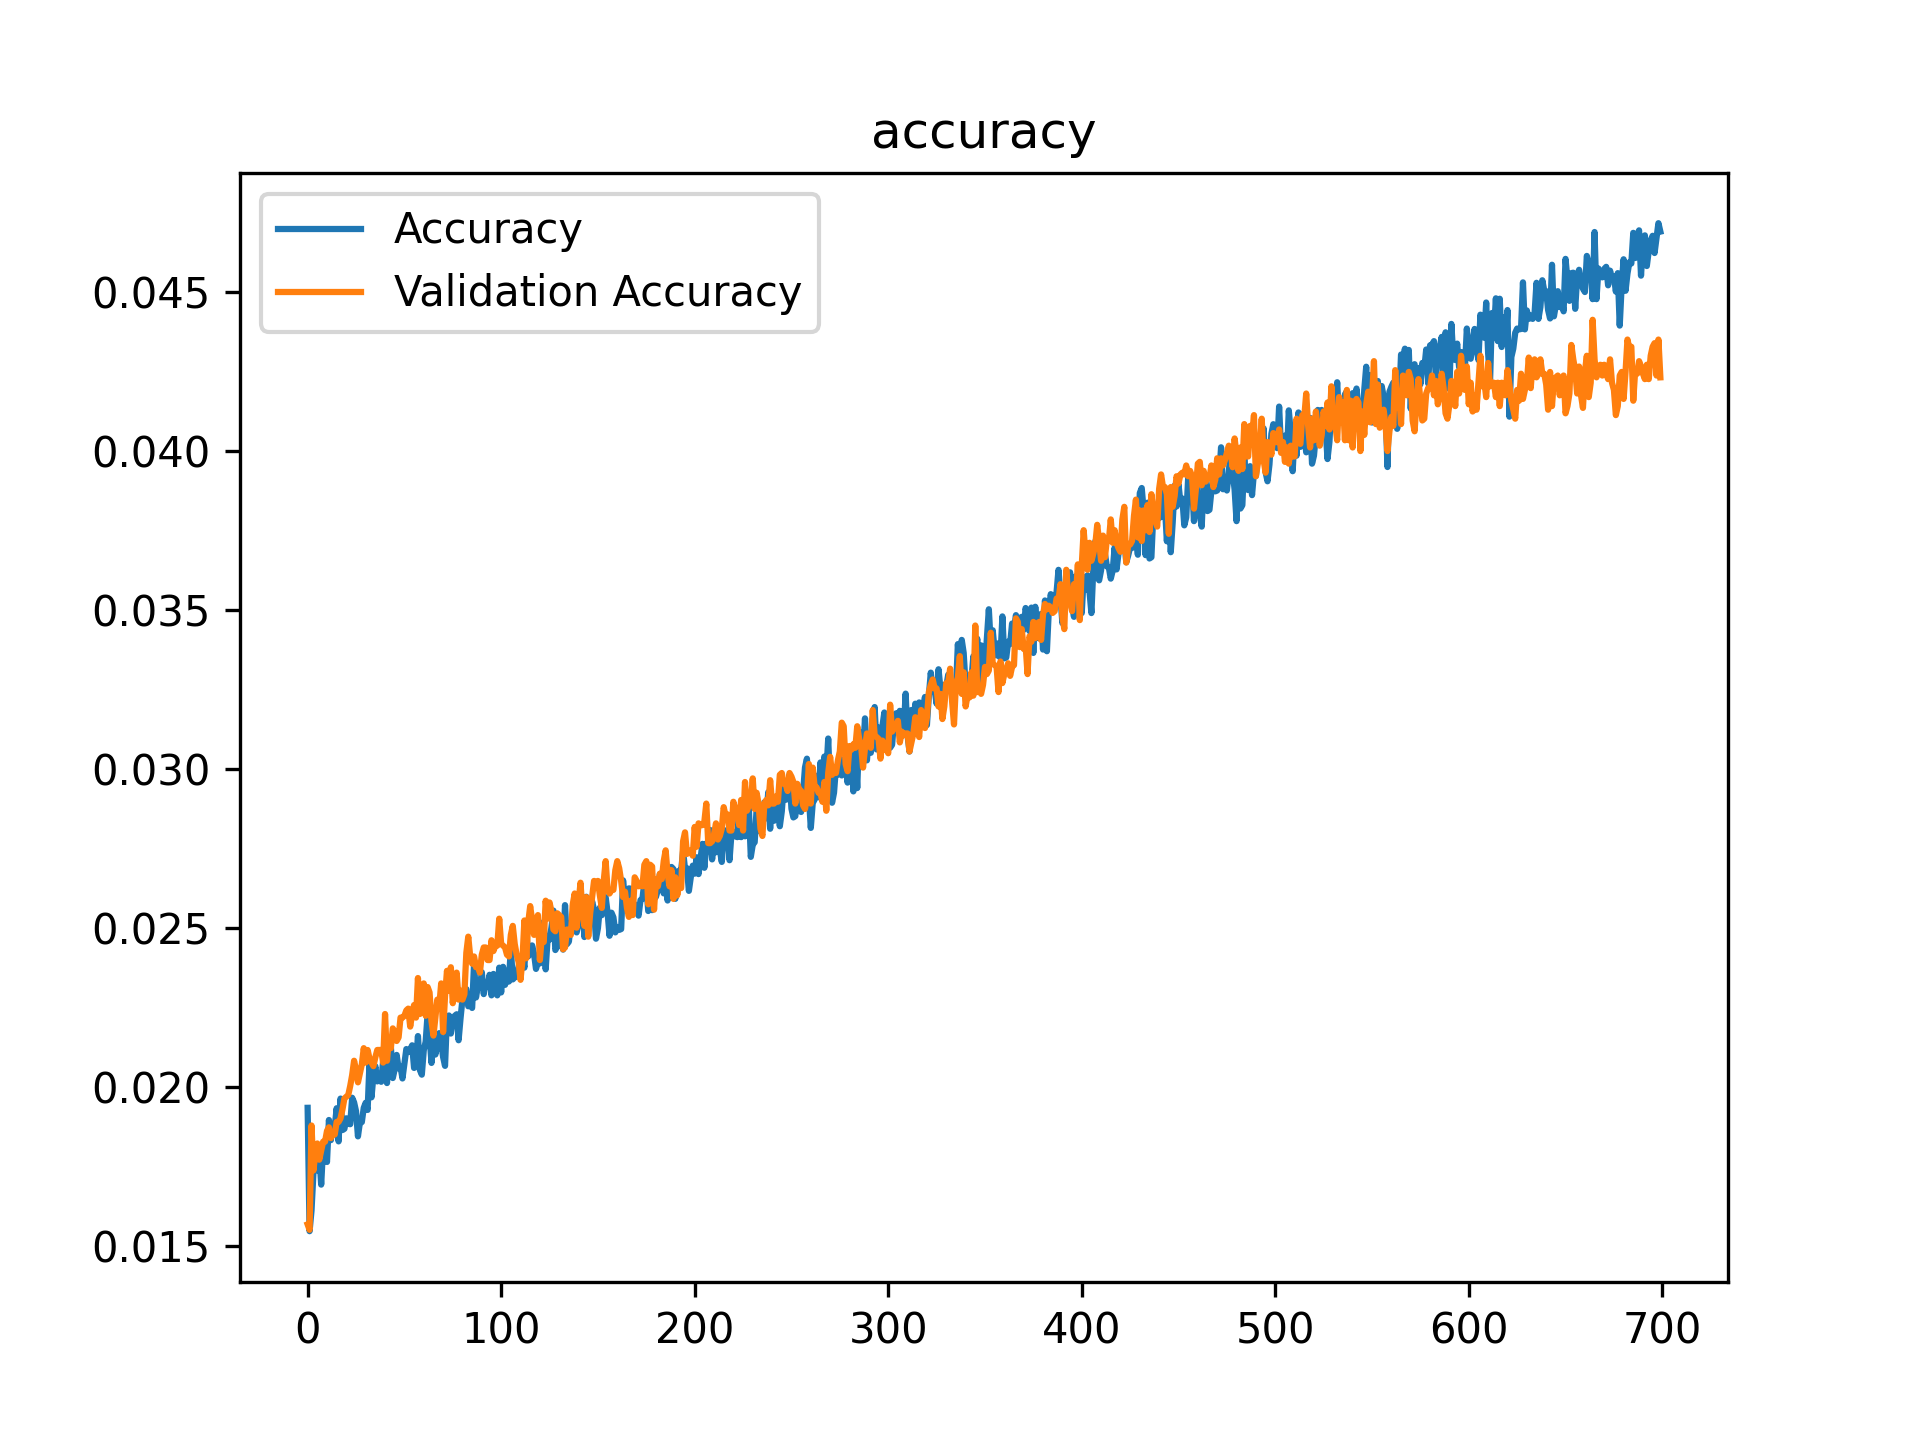
\includegraphics[width=1\linewidth]{recursos/imagens/results/food_accuracy2.png}
         \caption{Bloco 4.}
         \label{results:fig:datasets:3.3}
     \end{subfigure}
     ~
     \begin{subfigure}[t]{0.45\textwidth}
         \centering
         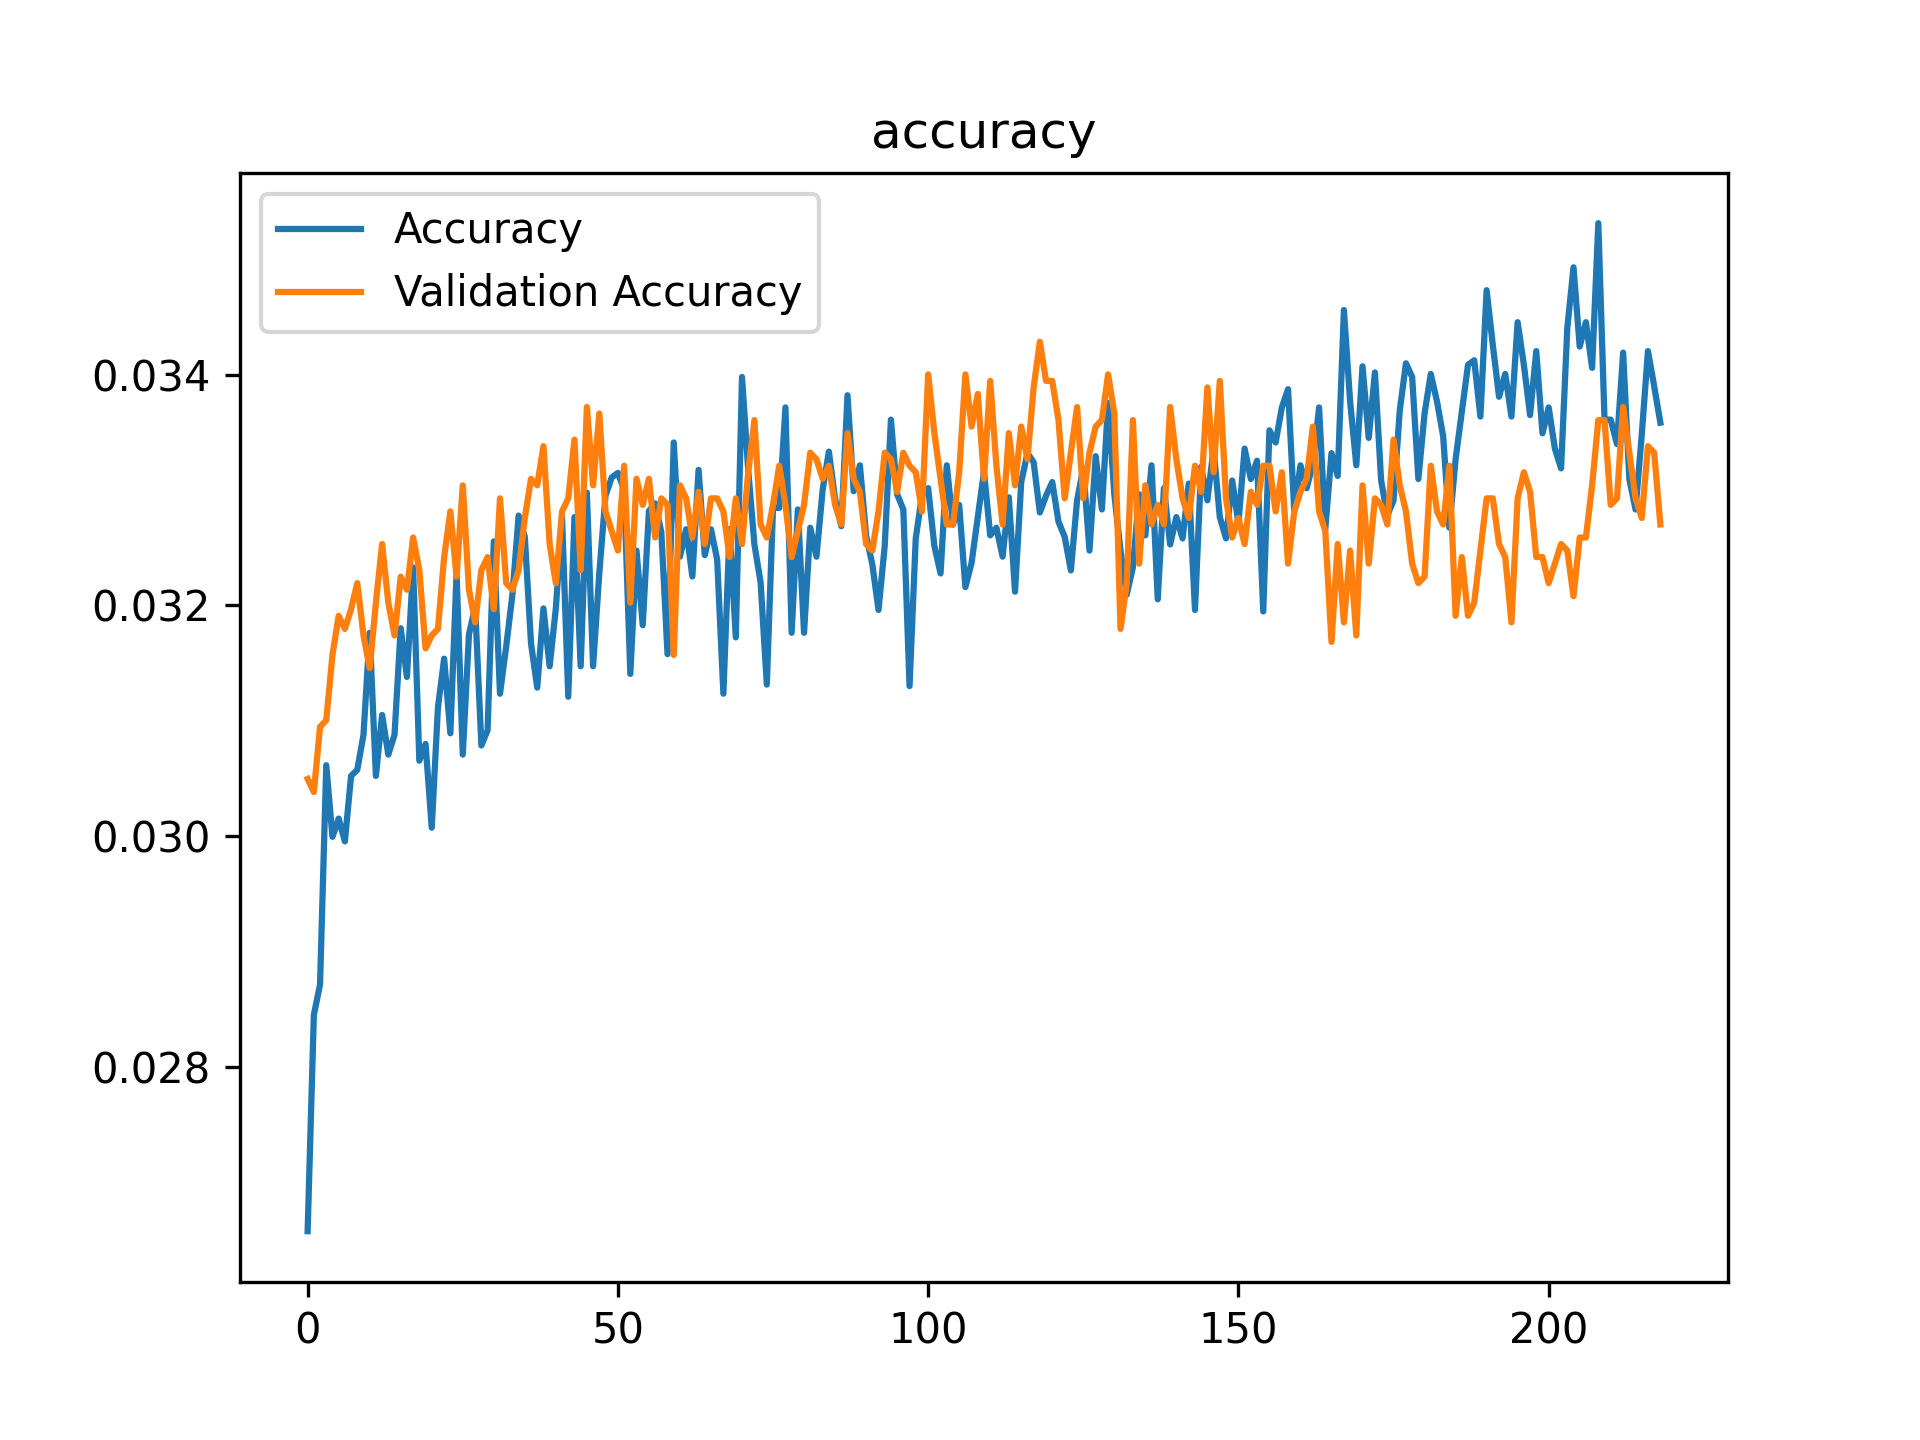
\includegraphics[width=1\linewidth]{recursos/imagens/results/food_accuracy3.png}
         \caption{Bloco 3.}
         \label{results:fig:datasets:3.4}
     \end{subfigure}
     
     Fonte: do próprio autor.
 \end{figure}

\begin{figure}[H]
    \centering
    \caption{Evolução da \textit{Loss} no conjunto de dados \textit{Food}-101.}
    \label{results:fig:datasets:4}
     \begin{subfigure}[t]{0.45\textwidth}
         \centering
         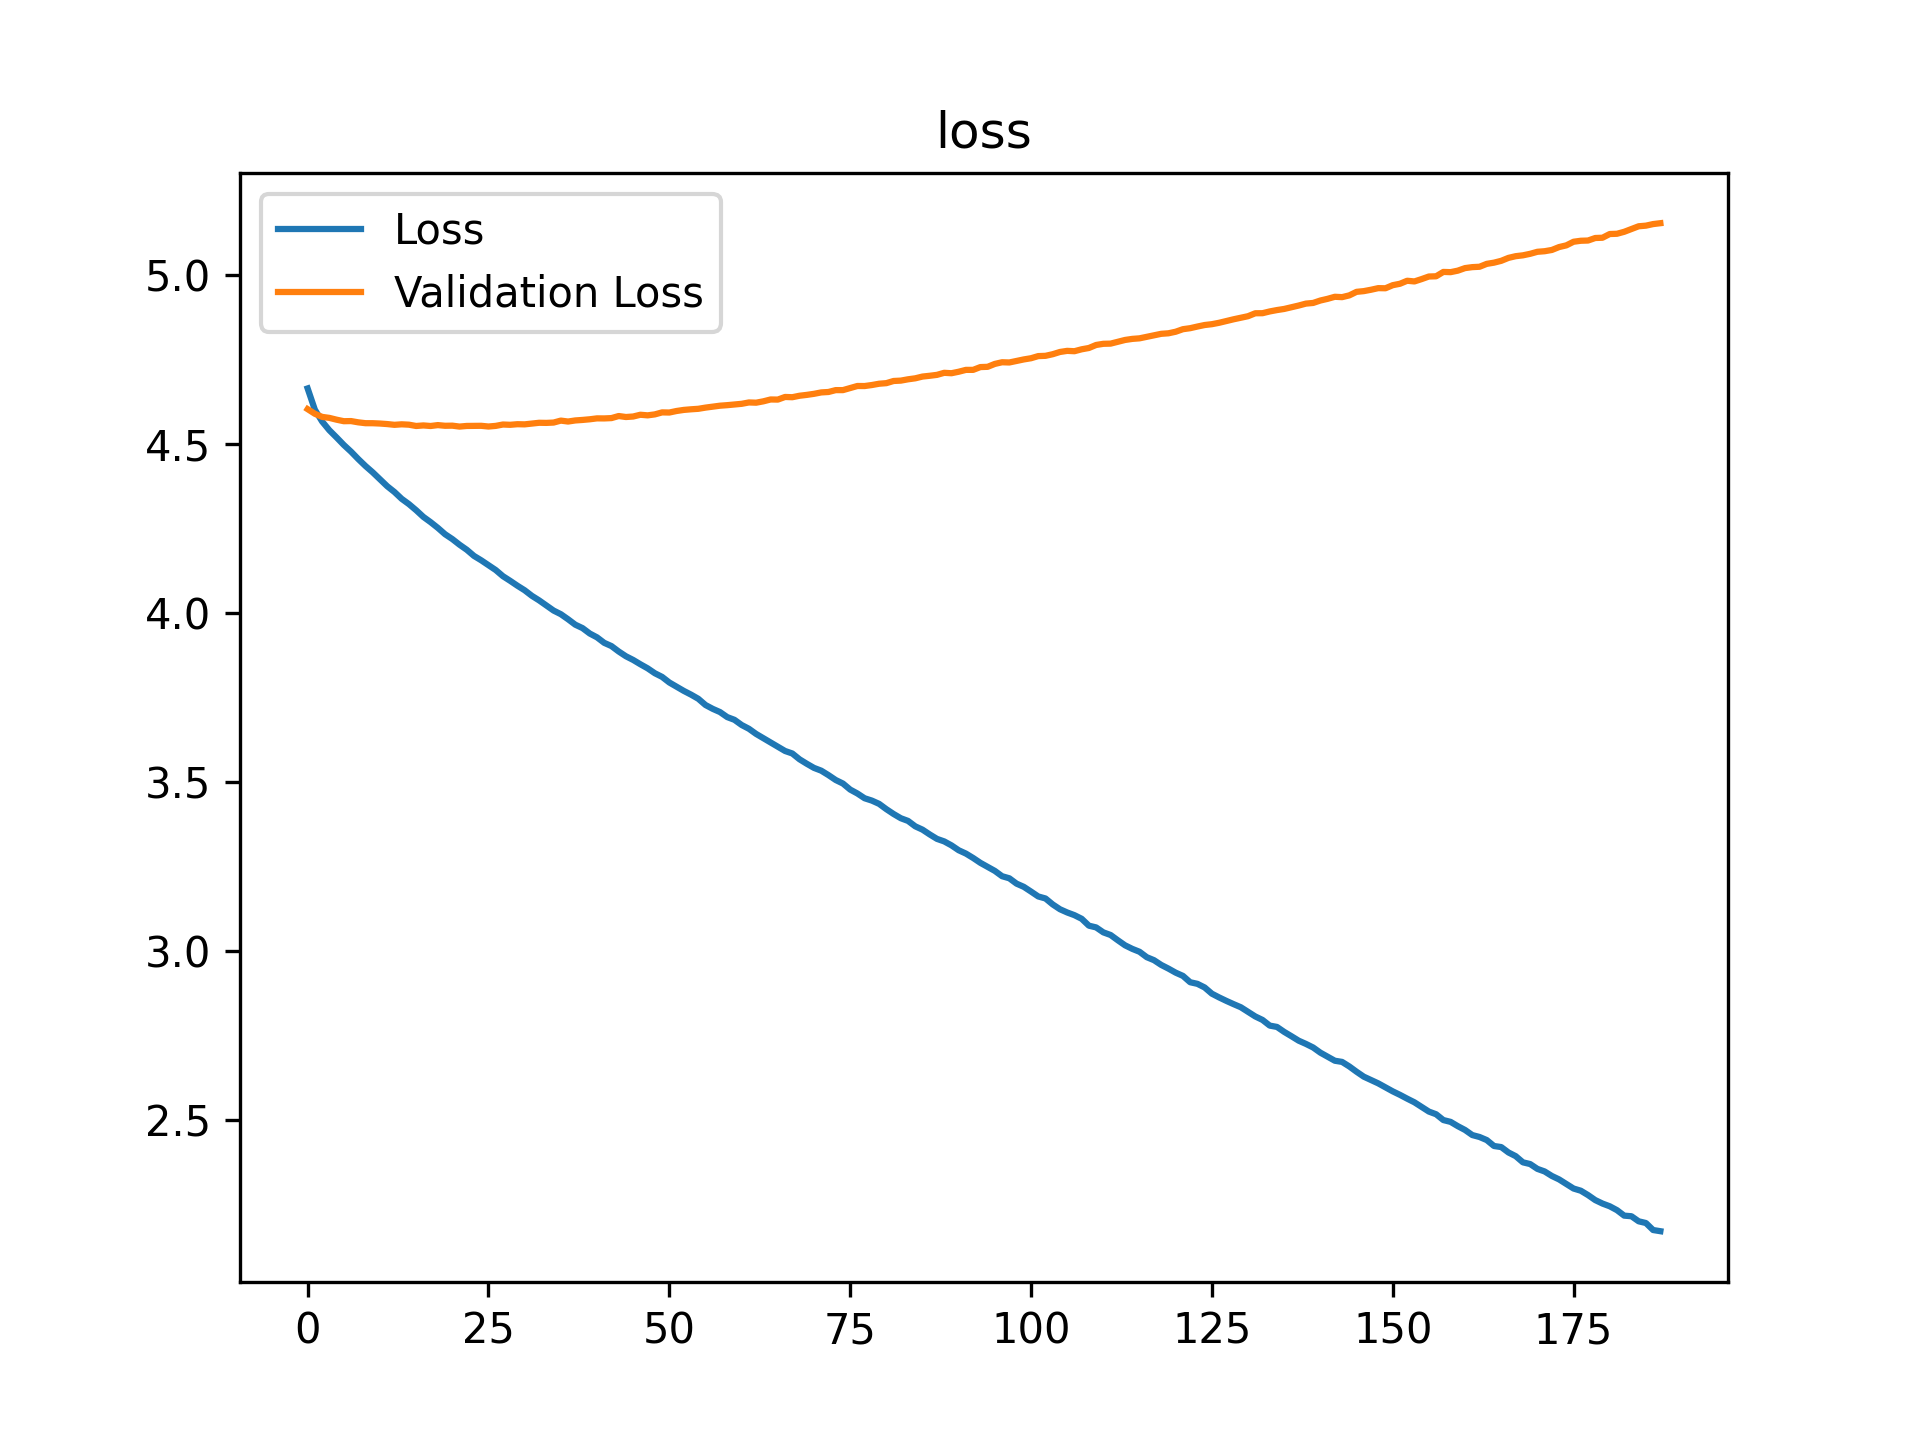
\includegraphics[width=1\linewidth]{recursos/imagens/results/food_wp_loss.png}
         \caption{Aquecimento.}
         \label{results:fig:datasets:4.1}
     \end{subfigure}%
     ~ 
     \begin{subfigure}[t]{0.45\textwidth}
         \centering
         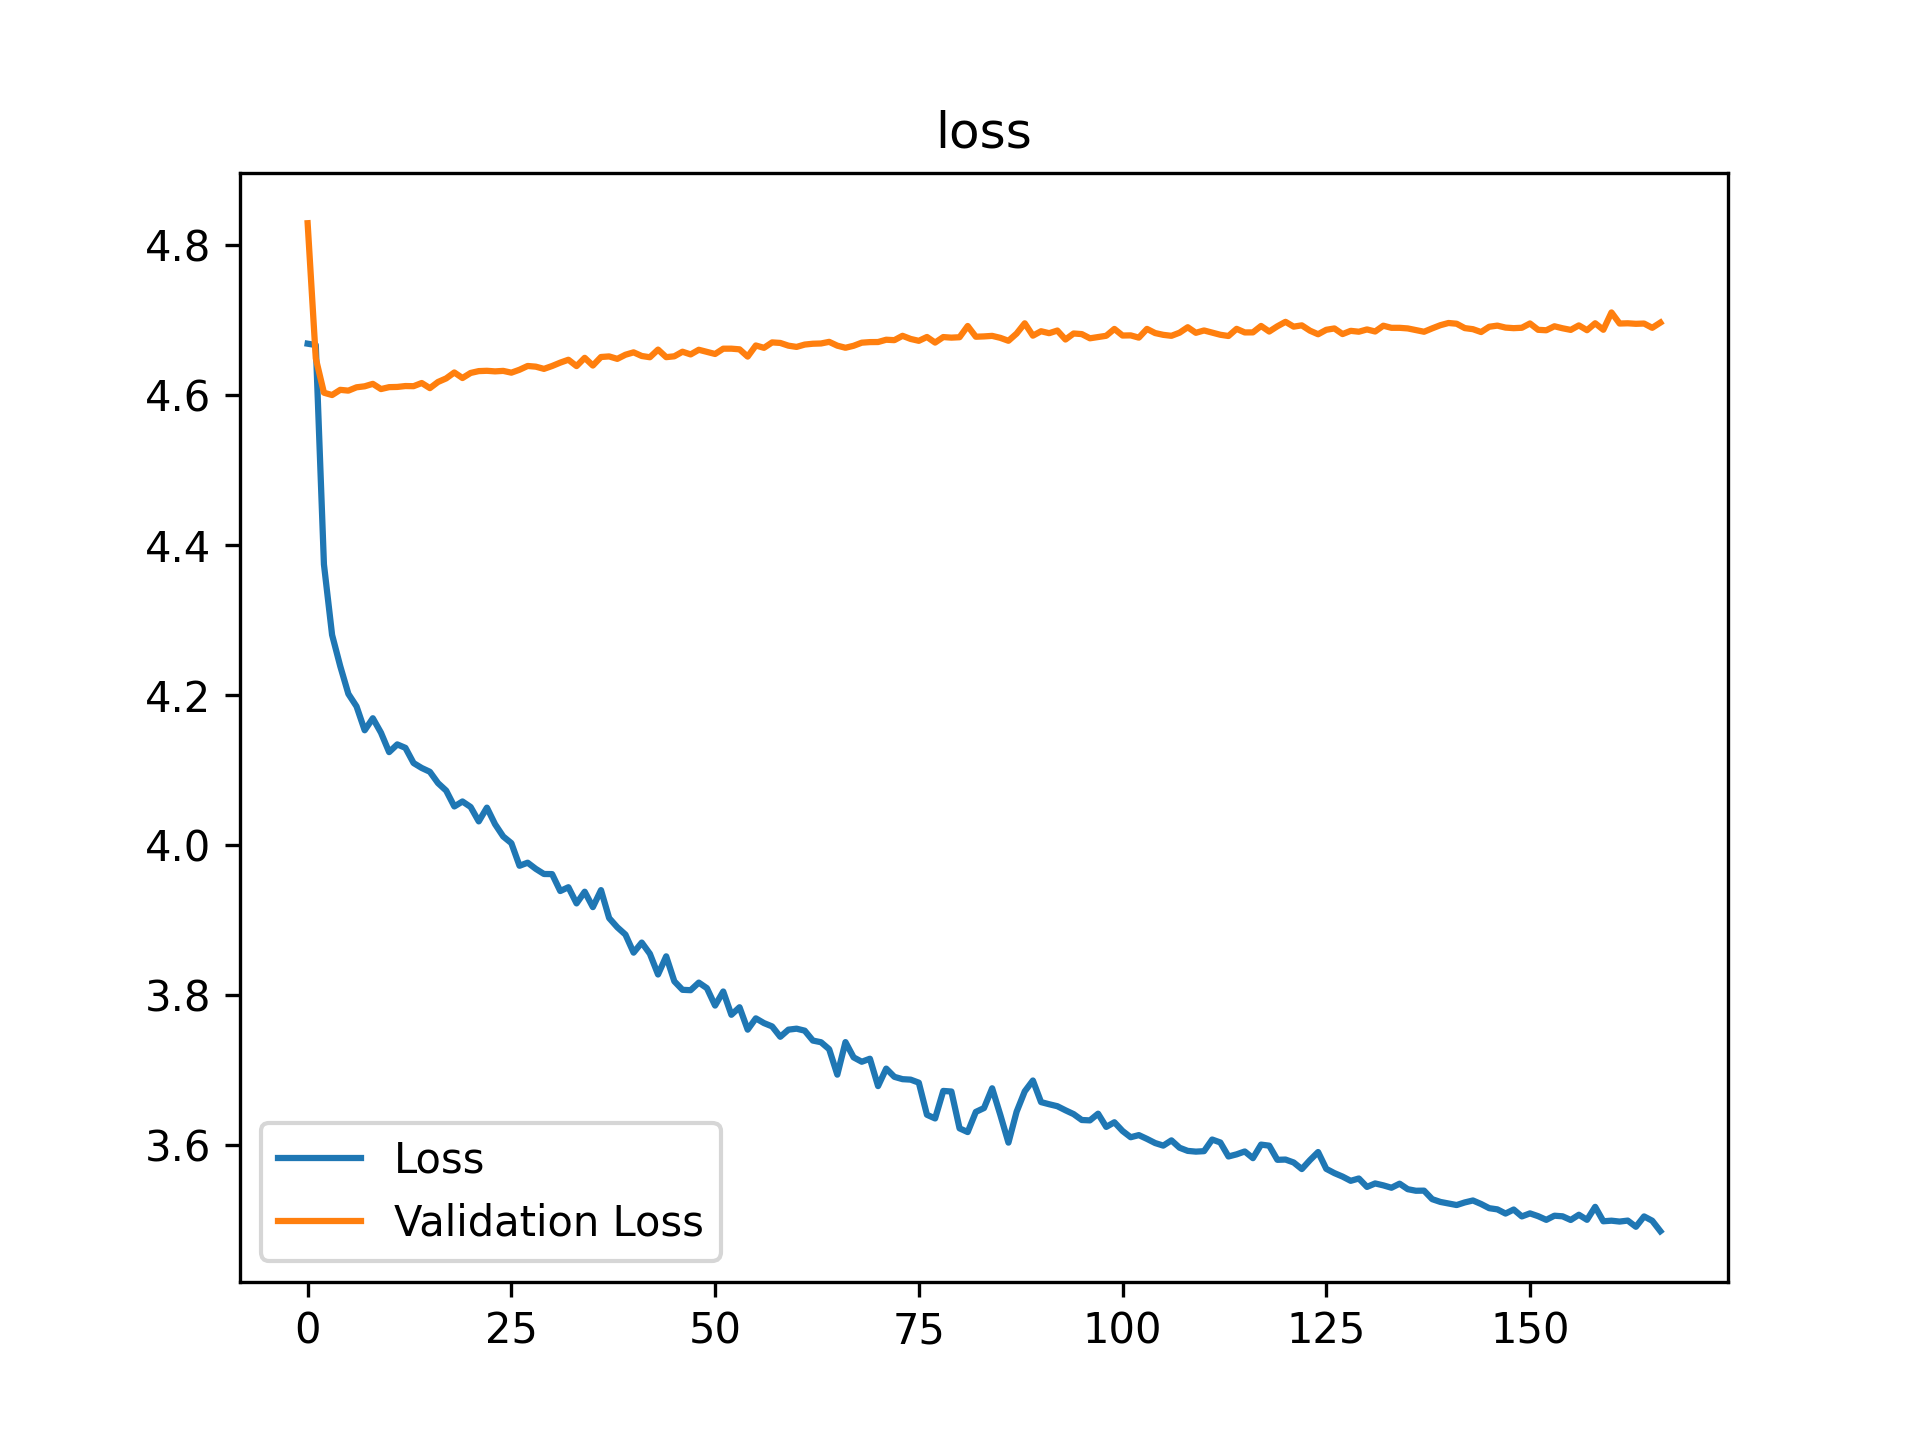
\includegraphics[width=1\linewidth]{recursos/imagens/results/food_loss1.png}
         \caption{Bloco 5.}
         \label{results:fig:datasets:4.2}
     \end{subfigure}%
     ~ 
     
     \begin{subfigure}[t]{0.45\textwidth}
         \centering
         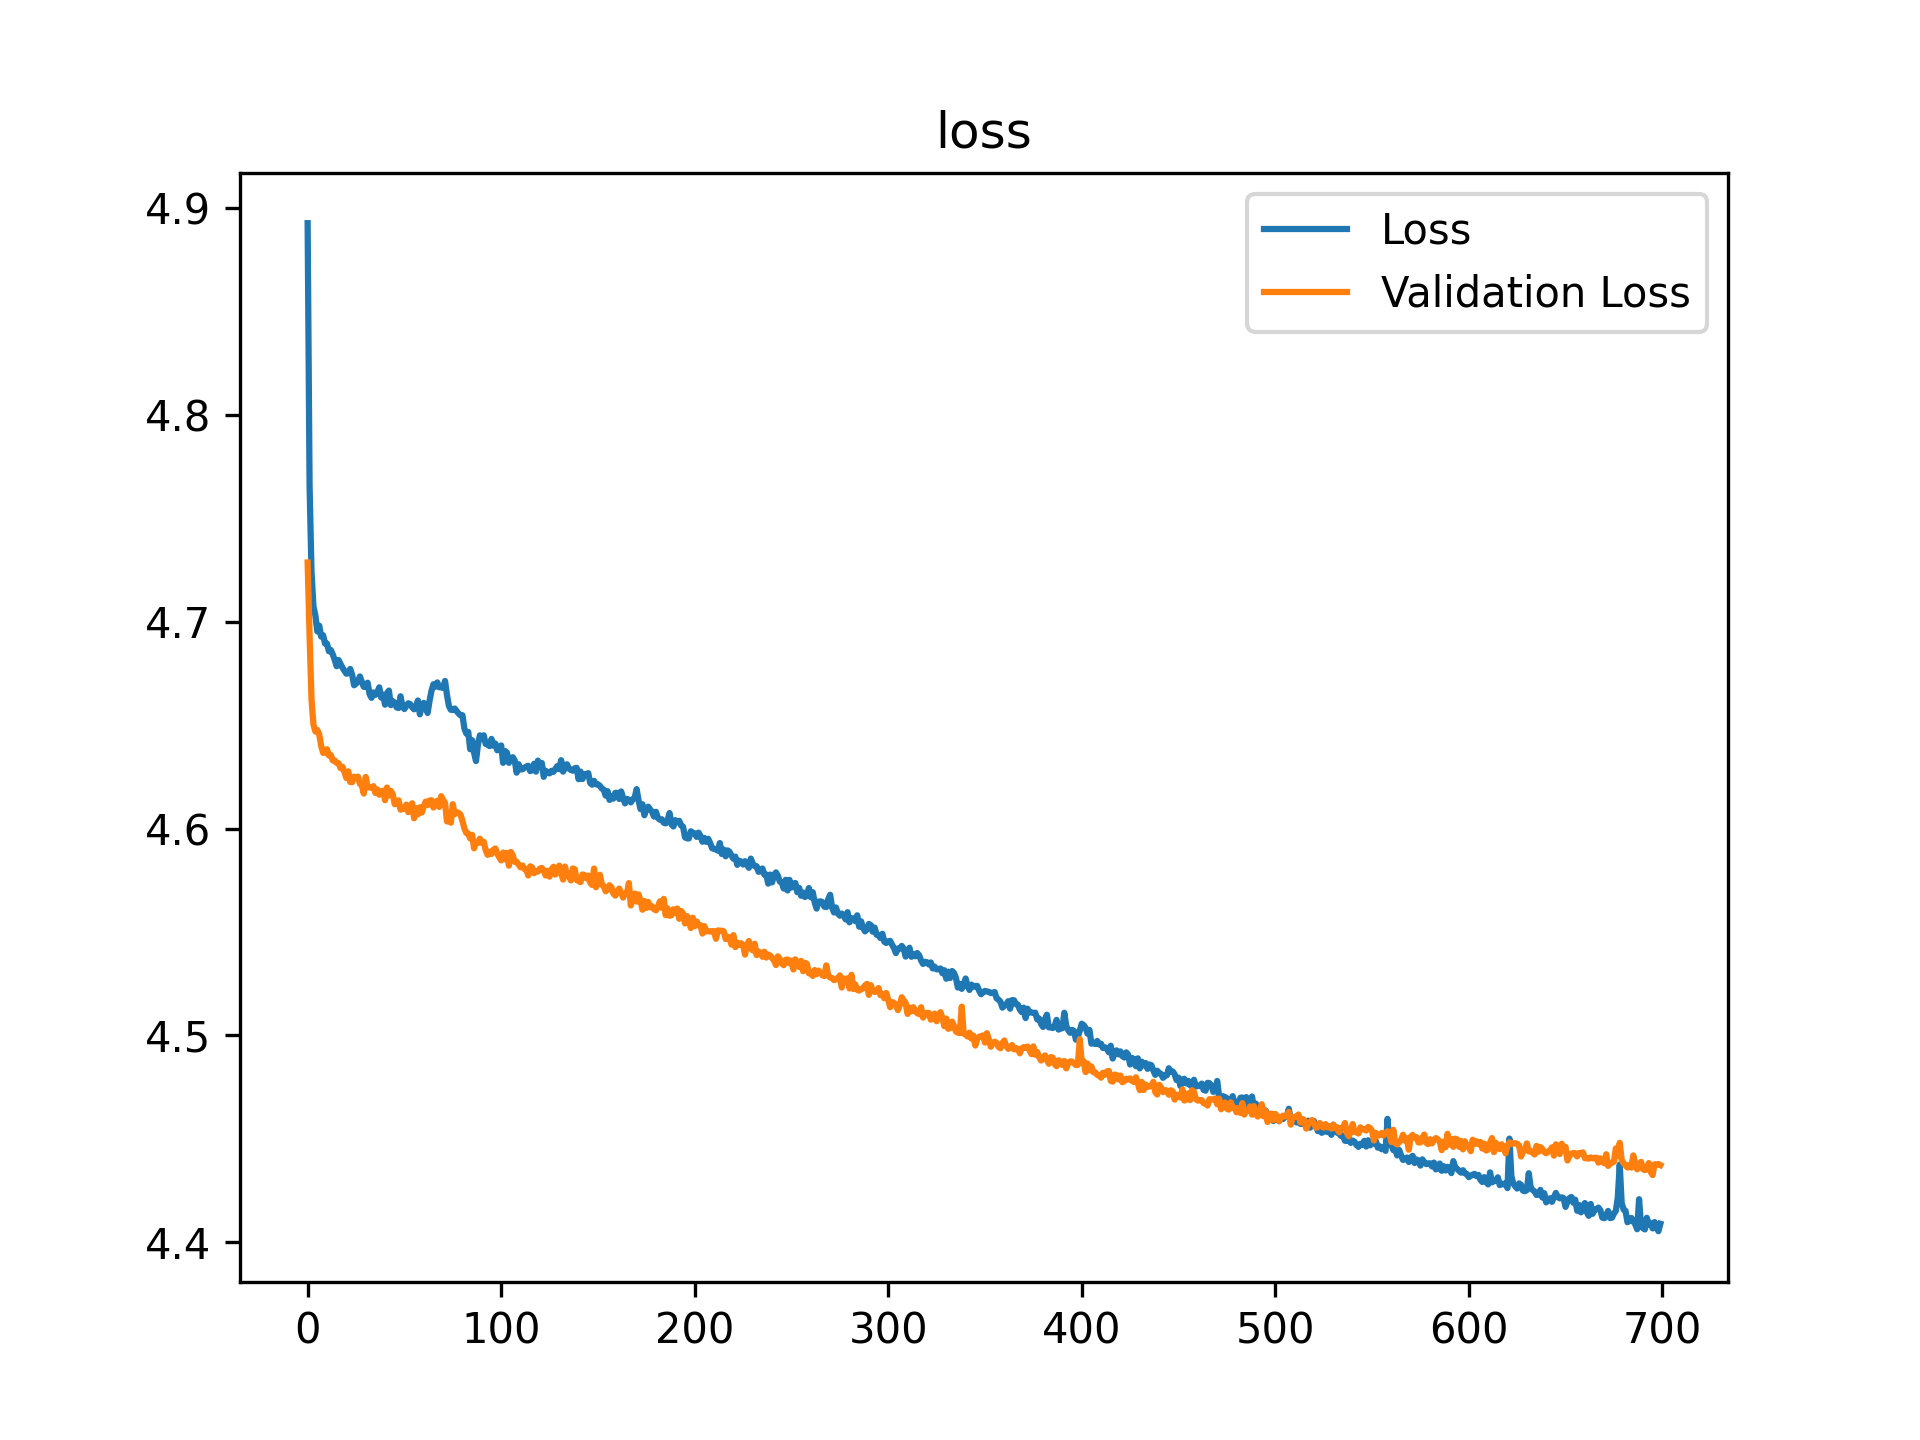
\includegraphics[width=1\linewidth]{recursos/imagens/results/food_loss2.png}
         \caption{Bloco 4.}
         \label{results:fig:datasets:4.3}
     \end{subfigure}
     ~
     \begin{subfigure}[t]{0.45\textwidth}
         \centering
         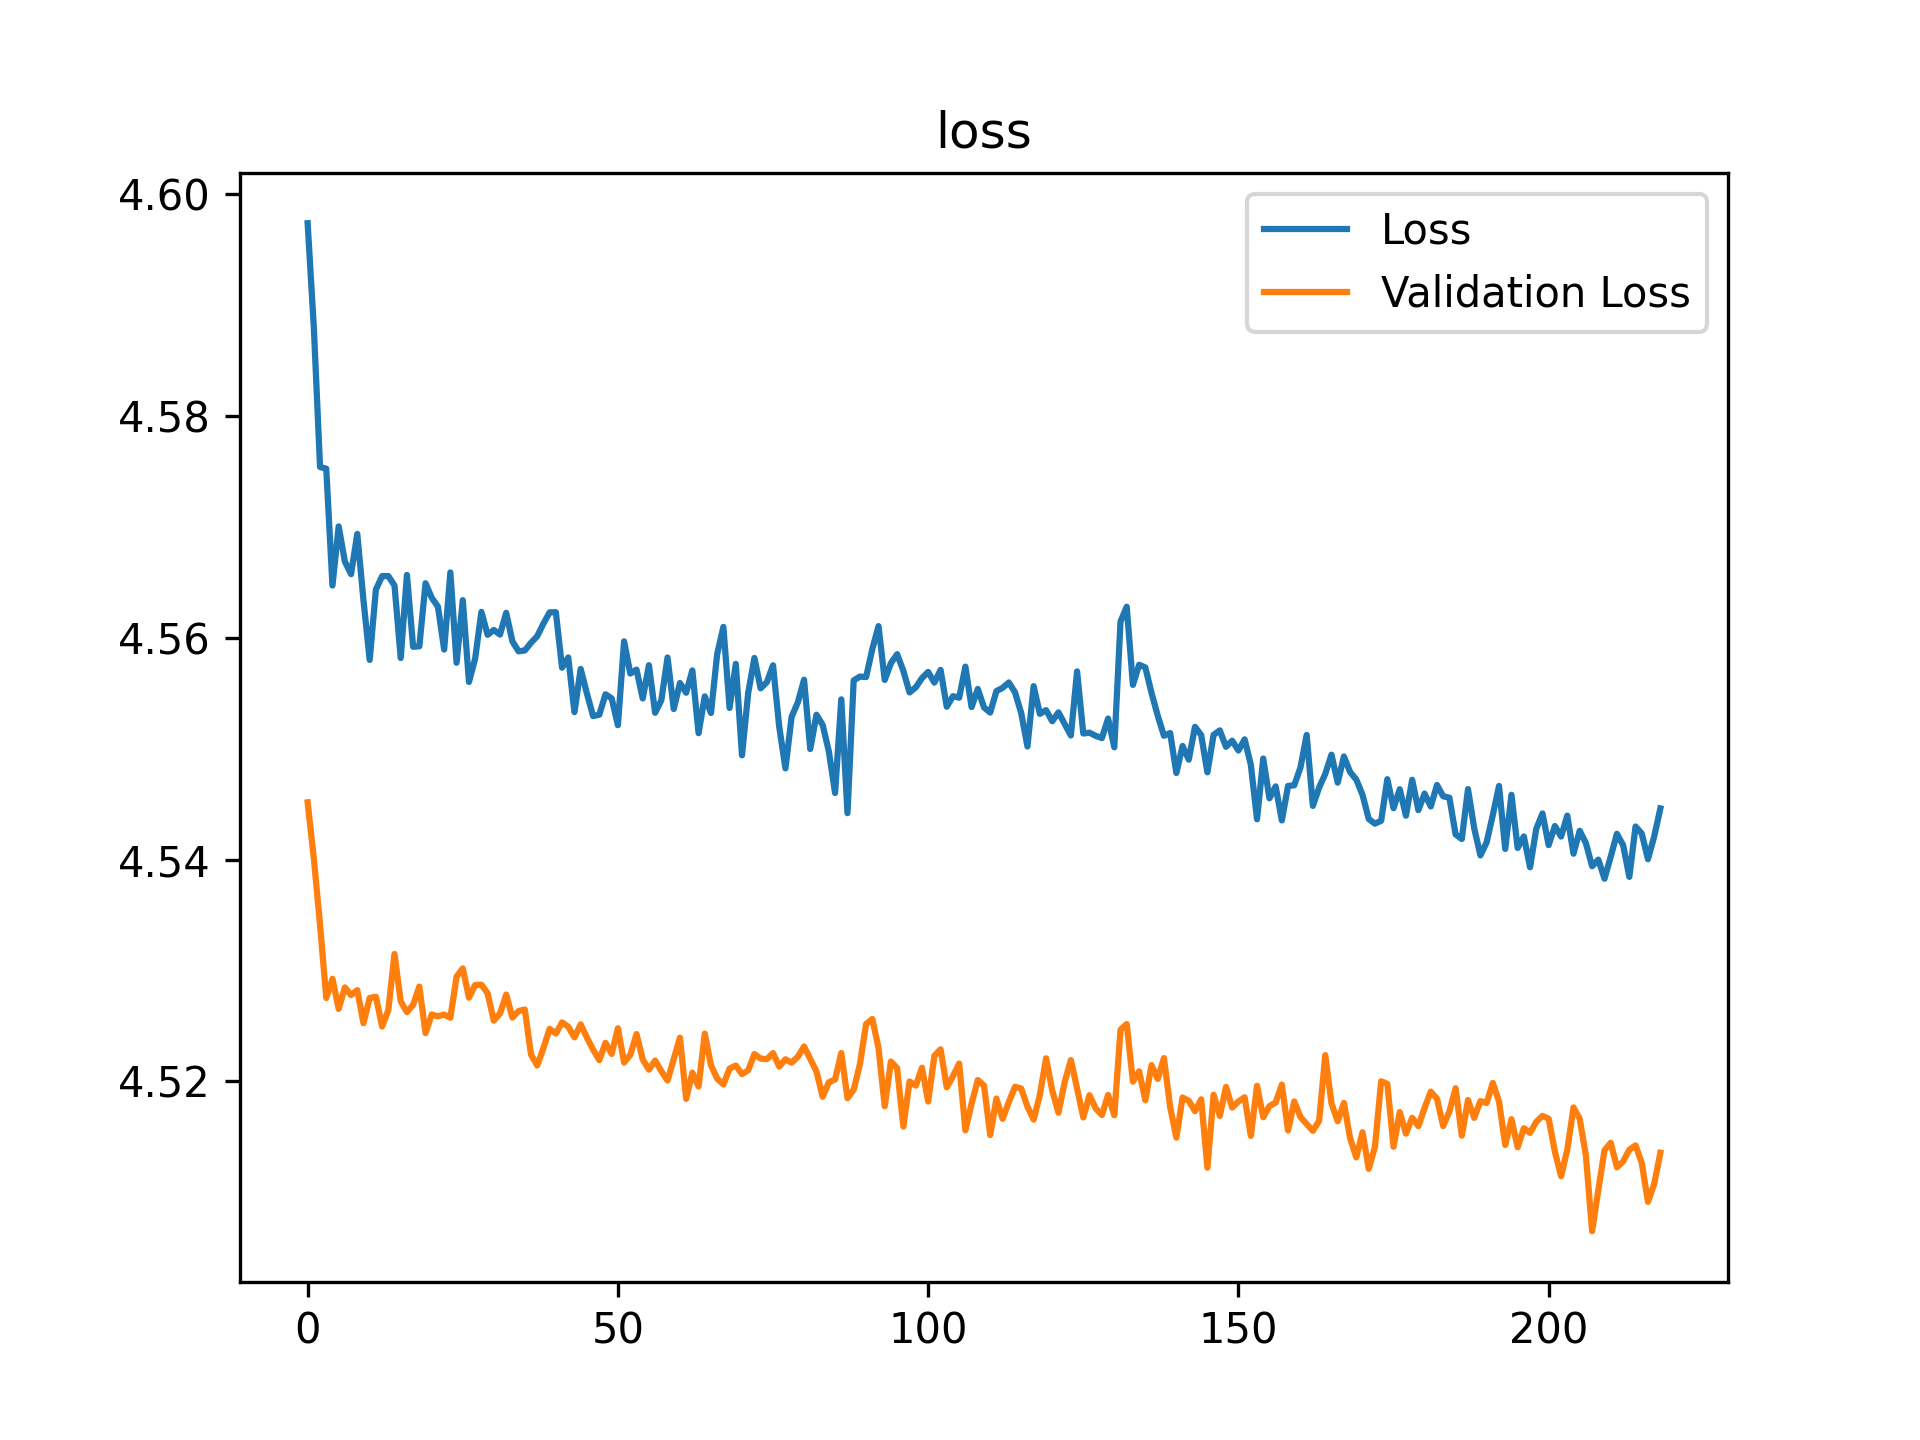
\includegraphics[width=1\linewidth]{recursos/imagens/results/food_loss3.png}
         \caption{Bloco 3.}
         \label{results:fig:datasets:4.4}
     \end{subfigure}
     
     Fonte: do próprio autor.
 \end{figure}

Em suma, a diversidade dos conjuntos de dados utilizados neste estudo forneceu uma avaliação robusta do método BPCAPooling, destacando tanto o seus pontos potenciais quanto a necessidade de otimizações específicas para diferentes cenários. As diferenças nos resultados reforçam a importância da seleção apropriada do conjunto de dados considerando suas características particulares.

\subsubsection{LIME e Preservação de Espacialidade}
\label{results:class:lime}
- Apresentar processo de preservação espacial, lime, fine tunning e custo computacional.

\subsubsection{Trabalhos Futuros}
\label{results:class:future}
Como mencionado na Seção \ref{project:transf}, os experimentos de classificação empregaram os princípios de transferência de aprendizado, o que comumente oferece vantagens devido ao reaproveitamento de pesos de arquiteturas treinadas em grandes conjuntos de dados \citep{Pan2010}. No entanto, embora as camadas de \textit{pooling} não tenham parâmetros treináveis diretamente afetados pela retro-propagação, elas influenciam diretamente as camadas de convolução subsequentes. Isso levanta a questão: \quotes{Será que o uso de transferência de aprendizado realmente contribuiu para a aplicação do método BPCAPooling nos experimentos realizados?} Uma vez que as camadas da rede passam a ficar com os pesos aquecidos, mas com o viés da utilização de um redutor de dimensionalidade que não mantém espacialidade, como é o caso do \textit{Max Pooling} e \textit{Avg Pooling}.

Além disso, outra questão pendente diz respeito a quais camadas precisam ser descongeladas para obter os melhores resultados possíveis com o método, já que investir em camadas associadas aos conceitos de espacialidade parece ser uma estratégia promissora, como comentado na Seção \ref{results:class:datasets}, que demonstra maior progresso no quarto bloco convolucional.

Por fim, a complexidade do método proposto é uma limitação. Um teste realizado com a arquitetura EfficientNetB0 \citep{Tan2019Efficientnet:Networks}, que possui $17$ camadas de \textit{pooling}, substituindo os métodos convencionais por BPCAPooling resultou em um tempo estimado de treinamento da fase de aquecimento de aproximadamente \textit{2.100} horas, de acordo com os padrões de desempenho comentados na Seção \ref{results:class}.

Para futuros trabalhos que visam aplicar o método BPCAPooling como camada de \textit{pooling} para arquiteturas de classificação, sugere-se a não utilização de transferência de aprendizado para o método, mas sim a realização de fases de treinamento e validação mais extensas, além do uso de conjuntos de dados equivalentes ao ImageNet, o que é um desafio devido às necessidades de \textit{hardware} que surgiriam. Uma sugestão adicional seria propor alternativas para otimizar a complexidade do código associado ao método BPCAPooling. Por fim, uma terceira ideia para trabalhos futuros, que também exigiria considerações sobre o \textit{hardware} necessário para os experimentos, seria a aplicação de mais épocas no descongelamento de determinados blocos convolucionais durante o processo de \textit{fine-tuning}, visando permitir a exploração mais profunda dos mapas de características e potencializar os aspectos de preservação espacial.

\subsection{Resultados da Segmentação Semântica}
\label{results:semantic}
- Colocar imagem para cada um dos resultados dos modelos e falar sobre a baixa diferença visualmente falando (falar que a diferença será relatada na seção \ref{results:semantic:xai})
- Não há uma discrepância significativa em relação às métricas quando comparado com max pooling, mas se apresenta mais lento e ainda tem menores métricas.
- Na prática em relação não tem muita mudança no resultado final exceto pelo tempo, complexidade e baixa acurácia

\subsubsection{Diferença das arquiteturas}
\label{results:semantic:arch}
- O treinamento com U-Net-Like realmente ocorrem mais rápido do que as U-Nets convencionais, visto que a quantidade de parâmetros é menor e as normalizações de batch normalization e convolução separáveis trazem o beneficio das otimizações.

\subsubsection{Explicação de modelos}
\label{results:semantic:xai}
- Colocar imagens comparando, mostrar os pontos de maior diferença para BPCA e Max Pooling.

\subsubsection{Trabalhos Futuros}
\label{results:semantic:future}
- Propor o uso de outro framework como pytorch e falar dos problemas tecnicamente enfrentados.
- Valeria um teste com outros datasets contendo objetos de diversos tamanhos, como lost and found, cityscape ou celulas. Mas a adaptação de código com o framework tensforflow se torna custosa, valeria a migração para o pytorch tentando minimizar essa barreira tecnológica.
- Valeria a implementação de um método de unpooling com o processo reverso de bpca (colocar a fórmula e imagens (repo compartilhado com uemerson)), a diferença é que esse método contaria com parâmetros, sendo necessário usar uma camada densa por baixo dos panos.


\subsection{Considerações Finais do Capítulo}
\label{result:final}
